% Options for packages loaded elsewhere
\PassOptionsToPackage{unicode}{hyperref}
\PassOptionsToPackage{hyphens}{url}
%
\documentclass[
]{article}
\usepackage{amsmath,amssymb}
\usepackage{iftex}
\ifPDFTeX
  \usepackage[T1]{fontenc}
  \usepackage[utf8]{inputenc}
  \usepackage{textcomp} % provide euro and other symbols
\else % if luatex or xetex
  \usepackage{unicode-math} % this also loads fontspec
  \defaultfontfeatures{Scale=MatchLowercase}
  \defaultfontfeatures[\rmfamily]{Ligatures=TeX,Scale=1}
\fi
\usepackage{lmodern}
\ifPDFTeX\else
  % xetex/luatex font selection
\fi
% Use upquote if available, for straight quotes in verbatim environments
\IfFileExists{upquote.sty}{\usepackage{upquote}}{}
\IfFileExists{microtype.sty}{% use microtype if available
  \usepackage[]{microtype}
  \UseMicrotypeSet[protrusion]{basicmath} % disable protrusion for tt fonts
}{}
\makeatletter
\@ifundefined{KOMAClassName}{% if non-KOMA class
  \IfFileExists{parskip.sty}{%
    \usepackage{parskip}
  }{% else
    \setlength{\parindent}{0pt}
    \setlength{\parskip}{6pt plus 2pt minus 1pt}}
}{% if KOMA class
  \KOMAoptions{parskip=half}}
\makeatother
\usepackage{xcolor}
\usepackage[margin=1in]{geometry}
\usepackage{color}
\usepackage{fancyvrb}
\newcommand{\VerbBar}{|}
\newcommand{\VERB}{\Verb[commandchars=\\\{\}]}
\DefineVerbatimEnvironment{Highlighting}{Verbatim}{commandchars=\\\{\}}
% Add ',fontsize=\small' for more characters per line
\usepackage{framed}
\definecolor{shadecolor}{RGB}{248,248,248}
\newenvironment{Shaded}{\begin{snugshade}}{\end{snugshade}}
\newcommand{\AlertTok}[1]{\textcolor[rgb]{0.94,0.16,0.16}{#1}}
\newcommand{\AnnotationTok}[1]{\textcolor[rgb]{0.56,0.35,0.01}{\textbf{\textit{#1}}}}
\newcommand{\AttributeTok}[1]{\textcolor[rgb]{0.13,0.29,0.53}{#1}}
\newcommand{\BaseNTok}[1]{\textcolor[rgb]{0.00,0.00,0.81}{#1}}
\newcommand{\BuiltInTok}[1]{#1}
\newcommand{\CharTok}[1]{\textcolor[rgb]{0.31,0.60,0.02}{#1}}
\newcommand{\CommentTok}[1]{\textcolor[rgb]{0.56,0.35,0.01}{\textit{#1}}}
\newcommand{\CommentVarTok}[1]{\textcolor[rgb]{0.56,0.35,0.01}{\textbf{\textit{#1}}}}
\newcommand{\ConstantTok}[1]{\textcolor[rgb]{0.56,0.35,0.01}{#1}}
\newcommand{\ControlFlowTok}[1]{\textcolor[rgb]{0.13,0.29,0.53}{\textbf{#1}}}
\newcommand{\DataTypeTok}[1]{\textcolor[rgb]{0.13,0.29,0.53}{#1}}
\newcommand{\DecValTok}[1]{\textcolor[rgb]{0.00,0.00,0.81}{#1}}
\newcommand{\DocumentationTok}[1]{\textcolor[rgb]{0.56,0.35,0.01}{\textbf{\textit{#1}}}}
\newcommand{\ErrorTok}[1]{\textcolor[rgb]{0.64,0.00,0.00}{\textbf{#1}}}
\newcommand{\ExtensionTok}[1]{#1}
\newcommand{\FloatTok}[1]{\textcolor[rgb]{0.00,0.00,0.81}{#1}}
\newcommand{\FunctionTok}[1]{\textcolor[rgb]{0.13,0.29,0.53}{\textbf{#1}}}
\newcommand{\ImportTok}[1]{#1}
\newcommand{\InformationTok}[1]{\textcolor[rgb]{0.56,0.35,0.01}{\textbf{\textit{#1}}}}
\newcommand{\KeywordTok}[1]{\textcolor[rgb]{0.13,0.29,0.53}{\textbf{#1}}}
\newcommand{\NormalTok}[1]{#1}
\newcommand{\OperatorTok}[1]{\textcolor[rgb]{0.81,0.36,0.00}{\textbf{#1}}}
\newcommand{\OtherTok}[1]{\textcolor[rgb]{0.56,0.35,0.01}{#1}}
\newcommand{\PreprocessorTok}[1]{\textcolor[rgb]{0.56,0.35,0.01}{\textit{#1}}}
\newcommand{\RegionMarkerTok}[1]{#1}
\newcommand{\SpecialCharTok}[1]{\textcolor[rgb]{0.81,0.36,0.00}{\textbf{#1}}}
\newcommand{\SpecialStringTok}[1]{\textcolor[rgb]{0.31,0.60,0.02}{#1}}
\newcommand{\StringTok}[1]{\textcolor[rgb]{0.31,0.60,0.02}{#1}}
\newcommand{\VariableTok}[1]{\textcolor[rgb]{0.00,0.00,0.00}{#1}}
\newcommand{\VerbatimStringTok}[1]{\textcolor[rgb]{0.31,0.60,0.02}{#1}}
\newcommand{\WarningTok}[1]{\textcolor[rgb]{0.56,0.35,0.01}{\textbf{\textit{#1}}}}
\usepackage{graphicx}
\makeatletter
\newsavebox\pandoc@box
\newcommand*\pandocbounded[1]{% scales image to fit in text height/width
  \sbox\pandoc@box{#1}%
  \Gscale@div\@tempa{\textheight}{\dimexpr\ht\pandoc@box+\dp\pandoc@box\relax}%
  \Gscale@div\@tempb{\linewidth}{\wd\pandoc@box}%
  \ifdim\@tempb\p@<\@tempa\p@\let\@tempa\@tempb\fi% select the smaller of both
  \ifdim\@tempa\p@<\p@\scalebox{\@tempa}{\usebox\pandoc@box}%
  \else\usebox{\pandoc@box}%
  \fi%
}
% Set default figure placement to htbp
\def\fps@figure{htbp}
\makeatother
\setlength{\emergencystretch}{3em} % prevent overfull lines
\providecommand{\tightlist}{%
  \setlength{\itemsep}{0pt}\setlength{\parskip}{0pt}}
\setcounter{secnumdepth}{-\maxdimen} % remove section numbering
\usepackage{fontspec}
\setmainfont{SimSun}
\setsansfont{SimSun}
\setmonofont{SimSun}
\usepackage{titling}
\pretitle{\begin{center}\Huge\bfseries}
\posttitle{\par\end{center}\vskip 1em}
\preauthor{\begin{center}\large}
\postauthor{\end{center}}
\predate{\begin{center}\large}
\postdate{\end{center}}
\usepackage{bookmark}
\IfFileExists{xurl.sty}{\usepackage{xurl}}{} % add URL line breaks if available
\urlstyle{same}
\hypersetup{
  pdftitle={《对Design factors in mouse-tracking: What makes a difference的可重复性研究》},
  pdfauthor={曹钟文、孙睿忻、姜文彬、郭冰冰},
  hidelinks,
  pdfcreator={LaTeX via pandoc}}

\title{《对Design factors in mouse-tracking: What makes a
difference的可重复性研究》}
\author{曹钟文、孙睿忻、姜文彬、郭冰冰}
\date{2025年06月17日}

\begin{document}
\maketitle

\newpage

\begin{center}\rule{0.5\linewidth}{0.5pt}\end{center}

\section{数据预处理和环境配置}\label{ux6570ux636eux9884ux5904ux7406ux548cux73afux5883ux914dux7f6e}

\subsection{加载 R 包}\label{ux52a0ux8f7d-r-ux5305}

\begin{Shaded}
\begin{Highlighting}[]
\CommentTok{\# 加载所需的 R 包:mousetrap 用于鼠标轨迹分析,ggplot2 用于绘图,dplyr、tidyr 用于数据处理,}
\CommentTok{\# afex 和 MBESS 用于方差分析与效应量估计,ordinal 用于有序回归分析。}
\FunctionTok{library}\NormalTok{(mousetrap)}
\end{Highlighting}
\end{Shaded}

\begin{verbatim}
## Warning: package 'mousetrap' was built under R version 4.4.3
\end{verbatim}

\begin{Shaded}
\begin{Highlighting}[]
\FunctionTok{library}\NormalTok{(ggplot2)}
\end{Highlighting}
\end{Shaded}

\begin{verbatim}
## Warning: package 'ggplot2' was built under R version 4.4.3
\end{verbatim}

\begin{Shaded}
\begin{Highlighting}[]
\FunctionTok{library}\NormalTok{(dplyr)}
\end{Highlighting}
\end{Shaded}

\begin{verbatim}
## Warning: package 'dplyr' was built under R version 4.4.3
\end{verbatim}

\begin{Shaded}
\begin{Highlighting}[]
\FunctionTok{library}\NormalTok{(tidyr)}
\end{Highlighting}
\end{Shaded}

\begin{verbatim}
## Warning: package 'tidyr' was built under R version 4.4.3
\end{verbatim}

\begin{Shaded}
\begin{Highlighting}[]
\FunctionTok{library}\NormalTok{(afex)}
\end{Highlighting}
\end{Shaded}

\begin{verbatim}
## Warning: package 'afex' was built under R version 4.4.3
\end{verbatim}

\begin{verbatim}
## Warning: package 'lme4' was built under R version 4.4.3
\end{verbatim}

\begin{verbatim}
## Warning: package 'Matrix' was built under R version 4.4.3
\end{verbatim}

\begin{Shaded}
\begin{Highlighting}[]
\FunctionTok{library}\NormalTok{(MBESS)}
\end{Highlighting}
\end{Shaded}

\begin{verbatim}
## Warning: package 'MBESS' was built under R version 4.4.3
\end{verbatim}

\begin{Shaded}
\begin{Highlighting}[]
\FunctionTok{library}\NormalTok{(ordinal)}
\end{Highlighting}
\end{Shaded}

\begin{verbatim}
## Warning: package 'ordinal' was built under R version 4.4.3
\end{verbatim}

\begin{Shaded}
\begin{Highlighting}[]
\FunctionTok{library}\NormalTok{(emmeans)}
\end{Highlighting}
\end{Shaded}

\begin{verbatim}
## Warning: package 'emmeans' was built under R version 4.4.3
\end{verbatim}

\begin{Shaded}
\begin{Highlighting}[]
\FunctionTok{library}\NormalTok{(maps)}
\end{Highlighting}
\end{Shaded}

\begin{verbatim}
## Warning: package 'maps' was built under R version 4.4.3
\end{verbatim}

\begin{Shaded}
\begin{Highlighting}[]
\FunctionTok{options}\NormalTok{(}\AttributeTok{warn =} \SpecialCharTok{{-}}\DecValTok{1}\NormalTok{)  }\CommentTok{\# 关闭所有警告}
\end{Highlighting}
\end{Shaded}

\subsection{自定义 ggplot2
主题}\label{ux81eaux5b9aux4e49-ggplot2-ux4e3bux9898}

\begin{Shaded}
\begin{Highlighting}[]
\CommentTok{\# 设置 ggplot2 图形的主题,使图形更美观且更适合科研展示。}
\FunctionTok{theme\_set}\NormalTok{(}\FunctionTok{theme\_classic}\NormalTok{()}\SpecialCharTok{+} 
  \FunctionTok{theme}\NormalTok{(}
    \AttributeTok{axis.line =} \FunctionTok{element\_line}\NormalTok{(}\AttributeTok{colour =} \StringTok{"black"}\NormalTok{),}
    \AttributeTok{axis.ticks =} \FunctionTok{element\_line}\NormalTok{(}\AttributeTok{colour =} \StringTok{"black"}\NormalTok{),}
    \AttributeTok{axis.text =} \FunctionTok{element\_text}\NormalTok{(}\AttributeTok{colour =} \StringTok{"black"}\NormalTok{),}
    \AttributeTok{panel.border =} \FunctionTok{element\_rect}\NormalTok{(}\AttributeTok{colour =} \StringTok{"black"}\NormalTok{, }\AttributeTok{fill=}\ConstantTok{NA}\NormalTok{)}
\NormalTok{  ))}
\end{Highlighting}
\end{Shaded}

\subsection{自定义函数}\label{ux81eaux5b9aux4e49ux51fdux6570}

\begin{Shaded}
\begin{Highlighting}[]
\CommentTok{\# 自定义函数:计算偏 Eta 平方(partial eta{-}squared)及其置信区间,}
\CommentTok{\# 用于衡量方差分析中的效应量。}
\NormalTok{get\_partial\_etas }\OtherTok{\textless{}{-}} \ControlFlowTok{function}\NormalTok{(anova\_table, }\AttributeTok{conf.level=}\NormalTok{.}\DecValTok{90}\NormalTok{)\{}
\NormalTok{  partial\_etas }\OtherTok{\textless{}{-}} \FunctionTok{sapply}\NormalTok{(}\FunctionTok{row.names}\NormalTok{(anova\_table),}\ControlFlowTok{function}\NormalTok{(i)\{}
\NormalTok{    F }\OtherTok{\textless{}{-}}\NormalTok{ anova\_table[i,}\StringTok{"F"}\NormalTok{]}
\NormalTok{    df1 }\OtherTok{\textless{}{-}}\NormalTok{ anova\_table[i,}\StringTok{"num Df"}\NormalTok{]}
\NormalTok{    df2 }\OtherTok{\textless{}{-}}\NormalTok{ anova\_table[i,}\StringTok{"den Df"}\NormalTok{]}
\NormalTok{    ci }\OtherTok{\textless{}{-}} \FunctionTok{conf.limits.ncf}\NormalTok{(}\AttributeTok{F.value=}\NormalTok{F,}\AttributeTok{conf.level=}\NormalTok{conf.level,}\AttributeTok{df.1=}\NormalTok{df1,}\AttributeTok{df.2=}\NormalTok{df2)}
    \FunctionTok{return}\NormalTok{(}
      \FunctionTok{c}\NormalTok{(}\AttributeTok{pes=}\NormalTok{((F}\SpecialCharTok{*}\NormalTok{df1)}\SpecialCharTok{/}\NormalTok{(F}\SpecialCharTok{*}\NormalTok{df1}\SpecialCharTok{+}\NormalTok{df2)),}
        \AttributeTok{lower=}\NormalTok{ci}\SpecialCharTok{$}\NormalTok{Lower.Limit}\SpecialCharTok{/}\NormalTok{(ci}\SpecialCharTok{$}\NormalTok{Lower.Limit}\SpecialCharTok{+}\NormalTok{df1}\SpecialCharTok{+}\NormalTok{df2}\SpecialCharTok{+}\DecValTok{1}\NormalTok{),}
        \AttributeTok{upper=}\NormalTok{ci}\SpecialCharTok{$}\NormalTok{Upper.Limit}\SpecialCharTok{/}\NormalTok{(ci}\SpecialCharTok{$}\NormalTok{Upper.Limit}\SpecialCharTok{+}\NormalTok{df1}\SpecialCharTok{+}\NormalTok{df2}\SpecialCharTok{+}\DecValTok{1}\NormalTok{)))}
\NormalTok{  \})}
  \FunctionTok{return}\NormalTok{(}\FunctionTok{t}\NormalTok{(partial\_etas))}
\NormalTok{\}}
\end{Highlighting}
\end{Shaded}

\subsection{导入数据}\label{ux5bfcux5165ux6570ux636e}

\begin{Shaded}
\begin{Highlighting}[]
\CommentTok{\# 导入原始实验数据,并将 Condition 和 group 设置为因子类型,指定顺序。}
\NormalTok{raw\_data }\OtherTok{\textless{}{-}} \FunctionTok{read.csv}\NormalTok{(}\StringTok{"C:/Users/86139/Desktop/exp3.csv"}\NormalTok{)}
\NormalTok{raw\_data}\SpecialCharTok{$}\NormalTok{Typicality }\OtherTok{\textless{}{-}} \FunctionTok{factor}\NormalTok{(raw\_data}\SpecialCharTok{$}\NormalTok{Condition,}\AttributeTok{levels=}\FunctionTok{c}\NormalTok{(}\StringTok{"Typical"}\NormalTok{,}\StringTok{"Atypical"}\NormalTok{))}
\NormalTok{raw\_data}\SpecialCharTok{$}\NormalTok{group }\OtherTok{\textless{}{-}} \FunctionTok{factor}\NormalTok{(raw\_data}\SpecialCharTok{$}\NormalTok{group,}\AttributeTok{levels=}\FunctionTok{c}\NormalTok{(}\StringTok{"static"}\NormalTok{,}\StringTok{"rtmax"}\NormalTok{,}\StringTok{"initmax"}\NormalTok{,}\StringTok{"dynamic"}\NormalTok{))}
\end{Highlighting}
\end{Shaded}

\section{正确性分析 -
包括所有试次}\label{ux6b63ux786eux6027ux5206ux6790---ux5305ux62ecux6240ux6709ux8bd5ux6b21}

\subsection{每个条件的正确反应比例}\label{ux6bcfux4e2aux6761ux4ef6ux7684ux6b63ux786eux53cdux5e94ux6bd4ux4f8b}

\begin{Shaded}
\begin{Highlighting}[]
\CommentTok{\# 计算每组中正确反应的比例。}
\FunctionTok{with}\NormalTok{(raw\_data,}\FunctionTok{table}\NormalTok{(group, correct)}\SpecialCharTok{/}\FunctionTok{c}\NormalTok{(}\FunctionTok{table}\NormalTok{(group)))}
\end{Highlighting}
\end{Shaded}

\begin{verbatim}
##          correct
## group              0          1
##   static  0.05887600 0.94112400
##   rtmax   0.10877193 0.89122807
##   initmax 0.10287081 0.89712919
##   dynamic 0.06403509 0.93596491
\end{verbatim}

\subsection{卡方检验}\label{ux5361ux65b9ux68c0ux9a8c}

\begin{Shaded}
\begin{Highlighting}[]
\CommentTok{\# 使用卡方检验检验正确率是否在各组之间有显著差异。}
\FunctionTok{chisq.test}\NormalTok{(}\FunctionTok{with}\NormalTok{(raw\_data,}\FunctionTok{table}\NormalTok{(group, correct)),}\AttributeTok{correct =} \ConstantTok{FALSE}\NormalTok{)}
\end{Highlighting}
\end{Shaded}

\begin{verbatim}
## 
##  Pearson's Chi-squared test
## 
## data:  with(raw_data, table(group, correct))
## X-squared = 29.927, df = 3, p-value = 1.43e-06
\end{verbatim}

\subsection{广义线性混合模型}\label{ux5e7fux4e49ux7ebfux6027ux6df7ux5408ux6a21ux578b}

\begin{Shaded}
\begin{Highlighting}[]
\CommentTok{\# 使用 GLMM 检验 group 是否对正确率有影响,包含被试作为随机效应。}
\FunctionTok{contrasts}\NormalTok{(raw\_data}\SpecialCharTok{$}\NormalTok{group)}
\end{Highlighting}
\end{Shaded}

\begin{verbatim}
##         rtmax initmax dynamic
## static      0       0       0
## rtmax       1       0       0
## initmax     0       1       0
## dynamic     0       0       1
\end{verbatim}

\begin{Shaded}
\begin{Highlighting}[]
\FunctionTok{summary}\NormalTok{(}\FunctionTok{glmer}\NormalTok{(correct}\SpecialCharTok{\textasciitilde{}}\NormalTok{(}\DecValTok{1}\SpecialCharTok{|}\NormalTok{subject\_nr)}\SpecialCharTok{+}\NormalTok{group,}\AttributeTok{family=}\StringTok{"binomial"}\NormalTok{,}\AttributeTok{data=}\NormalTok{raw\_data))}
\end{Highlighting}
\end{Shaded}

\begin{verbatim}
## Generalized linear mixed model fit by maximum likelihood (Laplace
##   Approximation) [glmerMod]
##  Family: binomial  ( logit )
## Formula: correct ~ (1 | subject_nr) + group
##    Data: raw_data
## 
##      AIC      BIC   logLik deviance df.resid 
##   2642.0   2674.2  -1316.0   2632.0     4650 
## 
## Scaled residuals: 
##     Min      1Q  Median      3Q     Max 
## -4.3273  0.2066  0.2595  0.3245  0.5809 
## 
## Random effects:
##  Groups     Name        Variance Std.Dev.
##  subject_nr (Intercept) 0.386    0.6213  
## Number of obs: 4655, groups:  subject_nr, 245
## 
## Fixed effects:
##              Estimate Std. Error z value Pr(>|z|)    
## (Intercept)   2.94406    0.16032  18.363  < 2e-16 ***
## grouprtmax   -0.70835    0.20093  -3.525 0.000423 ***
## groupinitmax -0.61969    0.19836  -3.124 0.001784 ** 
## groupdynamic -0.09055    0.21484  -0.421 0.673407    
## ---
## Signif. codes:  0 '***' 0.001 '**' 0.01 '*' 0.05 '.' 0.1 ' ' 1
## 
## Correlation of Fixed Effects:
##             (Intr) grprtm grpntm
## grouprtmax  -0.761              
## groupinitmx -0.760  0.602       
## groupdynamc -0.694  0.554  0.560
\end{verbatim}

\section{正确性分析 - 排除 rtmax
条件下超时试次}\label{ux6b63ux786eux6027ux5206ux6790---ux6392ux9664-rtmax-ux6761ux4ef6ux4e0bux8d85ux65f6ux8bd5ux6b21}

\subsection{排除超时试次}\label{ux6392ux9664ux8d85ux65f6ux8bd5ux6b21}

\begin{Shaded}
\begin{Highlighting}[]
\CommentTok{\# 计算 rtmax 条件下响应为 None(超时)的试次数量和比例。}
\NormalTok{n\_eligible }\OtherTok{\textless{}{-}} \FunctionTok{sum}\NormalTok{(}\FunctionTok{with}\NormalTok{(raw\_data,group}\SpecialCharTok{==}\StringTok{"rtmax"} \SpecialCharTok{\&}\NormalTok{ response}\SpecialCharTok{!=}\StringTok{"None"}\NormalTok{))}
\NormalTok{n\_noneligible }\OtherTok{\textless{}{-}} \FunctionTok{sum}\NormalTok{(}\FunctionTok{with}\NormalTok{(raw\_data,group}\SpecialCharTok{==}\StringTok{"rtmax"} \SpecialCharTok{\&}\NormalTok{ response}\SpecialCharTok{==}\StringTok{"None"}\NormalTok{))}
\NormalTok{n\_noneligible}\SpecialCharTok{/}\NormalTok{(n\_eligible}\SpecialCharTok{+}\NormalTok{n\_noneligible)}
\end{Highlighting}
\end{Shaded}

\begin{verbatim}
## [1] 0.0377193
\end{verbatim}

\begin{Shaded}
\begin{Highlighting}[]
\CommentTok{\# 删除超时的试次。}
\NormalTok{raw\_data }\OtherTok{\textless{}{-}} \FunctionTok{subset}\NormalTok{(raw\_data, response}\SpecialCharTok{!=}\StringTok{"None"}\NormalTok{)}
\end{Highlighting}
\end{Shaded}

\subsection{每个条件的正确反应比例(更新)}\label{ux6bcfux4e2aux6761ux4ef6ux7684ux6b63ux786eux53cdux5e94ux6bd4ux4f8bux66f4ux65b0}

\begin{Shaded}
\begin{Highlighting}[]
\CommentTok{\# 重新计算每组的正确率。}
\FunctionTok{with}\NormalTok{(raw\_data,}\FunctionTok{table}\NormalTok{(group, correct)}\SpecialCharTok{/}\FunctionTok{c}\NormalTok{(}\FunctionTok{table}\NormalTok{(group)))}
\end{Highlighting}
\end{Shaded}

\begin{verbatim}
##          correct
## group              0          1
##   static  0.05887600 0.94112400
##   rtmax   0.07383774 0.92616226
##   initmax 0.10287081 0.89712919
##   dynamic 0.06403509 0.93596491
\end{verbatim}

\subsection{卡方检验(更新)}\label{ux5361ux65b9ux68c0ux9a8cux66f4ux65b0}

\begin{Shaded}
\begin{Highlighting}[]
\CommentTok{\# 再次进行卡方检验。}
\FunctionTok{chisq.test}\NormalTok{(}\FunctionTok{with}\NormalTok{(raw\_data,}\FunctionTok{table}\NormalTok{(group, correct)),}\AttributeTok{correct =} \ConstantTok{FALSE}\NormalTok{)}
\end{Highlighting}
\end{Shaded}

\begin{verbatim}
## 
##  Pearson's Chi-squared test
## 
## data:  with(raw_data, table(group, correct))
## X-squared = 20.044, df = 3, p-value = 0.0001662
\end{verbatim}

\subsection{GLMM 模型(更新)}\label{glmm-ux6a21ux578bux66f4ux65b0}

\begin{Shaded}
\begin{Highlighting}[]
\CommentTok{\# 再次拟合 GLMM 模型,排除超时试次后的数据。}
\FunctionTok{summary}\NormalTok{(}\FunctionTok{glmer}\NormalTok{(correct}\SpecialCharTok{\textasciitilde{}}\NormalTok{(}\DecValTok{1}\SpecialCharTok{|}\NormalTok{subject\_nr)}\SpecialCharTok{+}\NormalTok{group,}\AttributeTok{family=}\StringTok{"binomial"}\NormalTok{,}\AttributeTok{data=}\NormalTok{raw\_data))}
\end{Highlighting}
\end{Shaded}

\begin{verbatim}
## Generalized linear mixed model fit by maximum likelihood (Laplace
##   Approximation) [glmerMod]
##  Family: binomial  ( logit )
## Formula: correct ~ (1 | subject_nr) + group
##    Data: raw_data
## 
##      AIC      BIC   logLik deviance df.resid 
##   2430.3   2462.5  -1210.2   2420.3     4607 
## 
## Scaled residuals: 
##     Min      1Q  Median      3Q     Max 
## -4.3768  0.1987  0.2359  0.2906  0.6089 
## 
## Random effects:
##  Groups     Name        Variance Std.Dev.
##  subject_nr (Intercept) 0.4761   0.69    
## Number of obs: 4612, groups:  subject_nr, 245
## 
## Fixed effects:
##              Estimate Std. Error z value Pr(>|z|)    
## (Intercept)    2.9800     0.1676  17.780  < 2e-16 ***
## grouprtmax    -0.2606     0.2204  -1.182  0.23716    
## groupinitmax  -0.6258     0.2073  -3.018  0.00254 ** 
## groupdynamic  -0.0915     0.2237  -0.409  0.68254    
## ---
## Signif. codes:  0 '***' 0.001 '**' 0.01 '*' 0.05 '.' 0.1 ' ' 1
## 
## Correlation of Fixed Effects:
##             (Intr) grprtm grpntm
## grouprtmax  -0.708              
## groupinitmx -0.756  0.567       
## groupdynamc -0.691  0.524  0.558
\end{verbatim}

\subsection{排除错误试次}\label{ux6392ux9664ux9519ux8befux8bd5ux6b21}

\begin{Shaded}
\begin{Highlighting}[]
\CommentTok{\# 进一步排除错误试次,只保留正确的反应。}
\NormalTok{raw\_data }\OtherTok{\textless{}{-}} \FunctionTok{subset}\NormalTok{(raw\_data, correct}\SpecialCharTok{==}\DecValTok{1}\NormalTok{)}
\end{Highlighting}
\end{Shaded}

\section{鼠标轨迹预处理}\label{ux9f20ux6807ux8f68ux8ff9ux9884ux5904ux7406}

\begin{Shaded}
\begin{Highlighting}[]
\CommentTok{\# 导入鼠标轨迹数据,进行坐标映射、起点对齐、导数计算、标准指标提取、时间标准化。}
\NormalTok{mt\_data }\OtherTok{\textless{}{-}} \FunctionTok{mt\_import\_mousetrap}\NormalTok{(raw\_data,}
  \AttributeTok{xpos\_label =} \FunctionTok{c}\NormalTok{(}\StringTok{"xpos\_initial\_phase"}\NormalTok{,}\StringTok{"xpos\_get\_response"}\NormalTok{),}
  \AttributeTok{ypos\_label =} \FunctionTok{c}\NormalTok{(}\StringTok{"ypos\_initial\_phase"}\NormalTok{,}\StringTok{"ypos\_get\_response"}\NormalTok{),}
  \AttributeTok{timestamps\_label =} \FunctionTok{c}\NormalTok{(}\StringTok{"timestamps\_initial\_phase"}\NormalTok{,}\StringTok{"timestamps\_get\_response"}\NormalTok{))}
\NormalTok{mt\_data }\OtherTok{\textless{}{-}} \FunctionTok{mt\_remap\_symmetric}\NormalTok{(mt\_data)}
\NormalTok{mt\_data }\OtherTok{\textless{}{-}} \FunctionTok{mt\_align\_start}\NormalTok{(mt\_data, }\AttributeTok{start=}\FunctionTok{c}\NormalTok{(}\DecValTok{0}\NormalTok{,}\DecValTok{0}\NormalTok{))}
\NormalTok{mt\_data }\OtherTok{\textless{}{-}} \FunctionTok{mt\_derivatives}\NormalTok{(mt\_data)}
\NormalTok{mt\_data }\OtherTok{\textless{}{-}} \FunctionTok{mt\_measures}\NormalTok{(mt\_data)}
\NormalTok{mt\_data }\OtherTok{\textless{}{-}} \FunctionTok{mt\_time\_normalize}\NormalTok{(mt\_data)}
\end{Highlighting}
\end{Shaded}

\section{操作检验(平均值)}\label{ux64cdux4f5cux68c0ux9a8cux5e73ux5747ux503c}

\subsection{聚合每位参与者的时间变量}\label{ux805aux5408ux6bcfux4f4dux53c2ux4e0eux8005ux7684ux65f6ux95f4ux53d8ux91cf}

\begin{Shaded}
\begin{Highlighting}[]
\CommentTok{\# 添加时间变量,并按被试聚合计算均值。}
\NormalTok{mt\_data}\SpecialCharTok{$}\NormalTok{measures}\SpecialCharTok{$}\NormalTok{RT\_initial }\OtherTok{\textless{}{-}}\NormalTok{ mt\_data}\SpecialCharTok{$}\NormalTok{data}\SpecialCharTok{$}\NormalTok{response\_time\_initial\_phase}
\NormalTok{mt\_data}\SpecialCharTok{$}\NormalTok{measures}\SpecialCharTok{$}\NormalTok{IT }\OtherTok{\textless{}{-}}\NormalTok{ mt\_data}\SpecialCharTok{$}\NormalTok{measures}\SpecialCharTok{$}\NormalTok{initiation\_time}
\NormalTok{mt\_data}\SpecialCharTok{$}\NormalTok{measures}\SpecialCharTok{$}\NormalTok{RT\_post }\OtherTok{\textless{}{-}}\NormalTok{ mt\_data}\SpecialCharTok{$}\NormalTok{data}\SpecialCharTok{$}\NormalTok{response\_time\_get\_response}

\NormalTok{agg\_times }\OtherTok{\textless{}{-}} \FunctionTok{mt\_aggregate\_per\_subject}\NormalTok{(mt\_data,}
  \AttributeTok{use\_variables =} \FunctionTok{c}\NormalTok{(}\StringTok{"RT\_initial"}\NormalTok{,}\StringTok{"IT"}\NormalTok{,}\StringTok{"RT"}\NormalTok{,}\StringTok{"RT\_post"}\NormalTok{),}
  \AttributeTok{use2\_variables =} \StringTok{"group"}\NormalTok{,}\AttributeTok{subject\_id=}\StringTok{"subject\_nr"}\NormalTok{)}
\end{Highlighting}
\end{Shaded}

\subsection{描述性统计}\label{ux63cfux8ff0ux6027ux7edfux8ba1}

\begin{Shaded}
\begin{Highlighting}[]
\CommentTok{\# 输出各组的均值和标准差。}
\NormalTok{mean\_times }\OtherTok{\textless{}{-}}\NormalTok{ agg\_times }\SpecialCharTok{\%\textgreater{}\%}
  \FunctionTok{group\_by}\NormalTok{(group) }\SpecialCharTok{\%\textgreater{}\%}
  \FunctionTok{summarize}\NormalTok{(}
    \AttributeTok{N =} \FunctionTok{n}\NormalTok{(),}
    \AttributeTok{M\_RT\_inital =} \FunctionTok{mean}\NormalTok{(RT\_initial),}
    \AttributeTok{SD\_RT\_initial =} \FunctionTok{sd}\NormalTok{(RT\_initial),}
    \AttributeTok{M\_IT =} \FunctionTok{mean}\NormalTok{(IT),}
    \AttributeTok{SD\_IT =} \FunctionTok{sd}\NormalTok{(IT),}
    \AttributeTok{M\_RT =} \FunctionTok{mean}\NormalTok{(RT),}
    \AttributeTok{SD\_RT =} \FunctionTok{sd}\NormalTok{(RT)}
\NormalTok{    ) }\SpecialCharTok{\%\textgreater{}\%}
  \FunctionTok{as.data.frame}\NormalTok{()}
\FunctionTok{print}\NormalTok{(mean\_times, }\AttributeTok{digits=}\DecValTok{5}\NormalTok{)}
\end{Highlighting}
\end{Shaded}

\begin{verbatim}
##     group  N M_RT_inital SD_RT_initial   M_IT  SD_IT   M_RT   SD_RT
## 1  static 59      808.47        324.06 508.69 215.60 2110.4  654.06
## 2   rtmax 60      650.12        176.61 437.25 159.98 1521.6  183.42
## 3 initmax 66      377.43        159.49 243.14 142.76 1471.7  248.62
## 4 dynamic 60      773.38        752.17 348.67 233.25 2805.4 1199.82
\end{verbatim}

\begin{Shaded}
\begin{Highlighting}[]
\CommentTok{\# 分析 RT\_post(动态条件)}
\NormalTok{agg\_times }\SpecialCharTok{\%\textgreater{}\%}
  \FunctionTok{group\_by}\NormalTok{(group) }\SpecialCharTok{\%\textgreater{}\%}
  \FunctionTok{summarize}\NormalTok{(}
    \AttributeTok{M\_RT\_post =} \FunctionTok{mean}\NormalTok{(RT\_post),}
    \AttributeTok{SD\_RT\_post =} \FunctionTok{sd}\NormalTok{(RT\_post)}
\NormalTok{  )}\SpecialCharTok{\%\textgreater{}\%}
  \FunctionTok{as.data.frame}\NormalTok{()}
\end{Highlighting}
\end{Shaded}

\begin{verbatim}
##     group M_RT_post SD_RT_post
## 1  static 1291.0419   584.8519
## 2   rtmax  860.5363   190.2649
## 3 initmax 1083.3367   308.9183
## 4 dynamic 2021.0729   671.1218
\end{verbatim}

\subsection{设置对比矩阵}\label{ux8bbeux7f6eux5bf9ux6bd4ux77e9ux9635}

\begin{Shaded}
\begin{Highlighting}[]
\CommentTok{\# 定义三种实验条件相对于 static 基线组的对比。}
\NormalTok{contrast\_matrix\_separate }\OtherTok{\textless{}{-}} \FunctionTok{list}\NormalTok{(}
  \AttributeTok{rtmax\_vs\_static =} \FunctionTok{c}\NormalTok{(}\SpecialCharTok{{-}}\DecValTok{1}\NormalTok{,}\DecValTok{1}\NormalTok{,}\DecValTok{0}\NormalTok{,}\DecValTok{0}\NormalTok{),}
  \AttributeTok{initmax\_vs\_static =} \FunctionTok{c}\NormalTok{(}\SpecialCharTok{{-}}\DecValTok{1}\NormalTok{,}\DecValTok{0}\NormalTok{,}\DecValTok{1}\NormalTok{,}\DecValTok{0}\NormalTok{),}
  \AttributeTok{dynamic\_vs\_static=} \FunctionTok{c}\NormalTok{(}\SpecialCharTok{{-}}\DecValTok{1}\NormalTok{,}\DecValTok{0}\NormalTok{,}\DecValTok{0}\NormalTok{,}\DecValTok{1}\NormalTok{))}
\end{Highlighting}
\end{Shaded}

\subsection{比较 RT\_initial}\label{ux6bd4ux8f83-rt_initial}

\begin{Shaded}
\begin{Highlighting}[]
\CommentTok{\# RT\_initial 的方差分析与对比分析。}
\NormalTok{anova\_RT\_initial }\OtherTok{\textless{}{-}} \FunctionTok{aov\_ez}\NormalTok{(}\AttributeTok{data=}\NormalTok{agg\_times,}\AttributeTok{dv =} \StringTok{"RT\_initial"}\NormalTok{, }\AttributeTok{between =} \StringTok{"group"}\NormalTok{, }\AttributeTok{id =} \StringTok{"subject\_nr"}\NormalTok{)}
\end{Highlighting}
\end{Shaded}

\begin{verbatim}
## Contrasts set to contr.sum for the following variables: group
\end{verbatim}

\begin{Shaded}
\begin{Highlighting}[]
\FunctionTok{nice}\NormalTok{(anova\_RT\_initial,}\AttributeTok{es =} \FunctionTok{c}\NormalTok{(}\StringTok{"pes"}\NormalTok{,}\StringTok{"ges"}\NormalTok{))}
\end{Highlighting}
\end{Shaded}

\begin{verbatim}
## Anova Table (Type 3 tests)
## 
## Response: RT_initial
##   Effect     df       MSE         F  ges  pes p.value
## 1  group 3, 241 178274.40 13.64 *** .145 .145   <.001
## ---
## Signif. codes:  0 '***' 0.001 '**' 0.01 '*' 0.05 '+' 0.1 ' ' 1
\end{verbatim}

\begin{Shaded}
\begin{Highlighting}[]
\FunctionTok{round}\NormalTok{(}\FunctionTok{get\_partial\_etas}\NormalTok{(anova\_RT\_initial}\SpecialCharTok{$}\NormalTok{anova\_table, }\AttributeTok{conf.level=}\NormalTok{.}\DecValTok{90}\NormalTok{),}\DecValTok{2}\NormalTok{)}
\end{Highlighting}
\end{Shaded}

\begin{verbatim}
##        pes lower upper
## group 0.15  0.08  0.21
\end{verbatim}

\begin{Shaded}
\begin{Highlighting}[]
\NormalTok{anova\_RT\_initial\_grid }\OtherTok{\textless{}{-}} \FunctionTok{lsmeans}\NormalTok{(anova\_RT\_initial,}\SpecialCharTok{\textasciitilde{}}\NormalTok{group)}
\FunctionTok{contrast}\NormalTok{(anova\_RT\_initial\_grid,contrast\_matrix\_separate)}
\end{Highlighting}
\end{Shaded}

\begin{verbatim}
##  contrast          estimate   SE  df t.ratio p.value
##  rtmax_vs_static     -158.4 77.4 241  -2.046  0.0419
##  initmax_vs_static   -431.0 75.6 241  -5.698  <.0001
##  dynamic_vs_static    -35.1 77.4 241  -0.453  0.6507
\end{verbatim}

\subsection{比较启动时间
IT}\label{ux6bd4ux8f83ux542fux52a8ux65f6ux95f4-it}

\begin{Shaded}
\begin{Highlighting}[]
\CommentTok{\# IT 的方差分析与对比分析。}
\NormalTok{anova\_IT }\OtherTok{\textless{}{-}} \FunctionTok{aov\_ez}\NormalTok{(}\AttributeTok{data=}\NormalTok{agg\_times,}\AttributeTok{dv =} \StringTok{"IT"}\NormalTok{, }\AttributeTok{between =} \StringTok{"group"}\NormalTok{, }\AttributeTok{id =} \StringTok{"subject\_nr"}\NormalTok{)}
\end{Highlighting}
\end{Shaded}

\begin{verbatim}
## Contrasts set to contr.sum for the following variables: group
\end{verbatim}

\begin{Shaded}
\begin{Highlighting}[]
\FunctionTok{nice}\NormalTok{(anova\_IT,}\AttributeTok{es =} \FunctionTok{c}\NormalTok{(}\StringTok{"pes"}\NormalTok{,}\StringTok{"ges"}\NormalTok{))}
\end{Highlighting}
\end{Shaded}

\begin{verbatim}
## Anova Table (Type 3 tests)
## 
## Response: IT
##   Effect     df      MSE         F  ges  pes p.value
## 1  group 3, 241 36268.60 22.69 *** .220 .220   <.001
## ---
## Signif. codes:  0 '***' 0.001 '**' 0.01 '*' 0.05 '+' 0.1 ' ' 1
\end{verbatim}

\begin{Shaded}
\begin{Highlighting}[]
\FunctionTok{round}\NormalTok{(}\FunctionTok{get\_partial\_etas}\NormalTok{(anova\_IT}\SpecialCharTok{$}\NormalTok{anova\_table, }\AttributeTok{conf.level=}\NormalTok{.}\DecValTok{90}\NormalTok{),}\DecValTok{2}\NormalTok{)}
\end{Highlighting}
\end{Shaded}

\begin{verbatim}
##        pes lower upper
## group 0.22  0.14  0.29
\end{verbatim}

\begin{Shaded}
\begin{Highlighting}[]
\NormalTok{anova\_IT\_grid }\OtherTok{\textless{}{-}} \FunctionTok{lsmeans}\NormalTok{(anova\_IT,}\SpecialCharTok{\textasciitilde{}}\NormalTok{group)}
\FunctionTok{contrast}\NormalTok{(anova\_IT\_grid,contrast\_matrix\_separate)}
\end{Highlighting}
\end{Shaded}

\begin{verbatim}
##  contrast          estimate   SE  df t.ratio p.value
##  rtmax_vs_static      -71.4 34.9 241  -2.046  0.0418
##  initmax_vs_static   -265.6 34.1 241  -7.783  <.0001
##  dynamic_vs_static   -160.0 34.9 241  -4.583  <.0001
\end{verbatim}

\subsection{比较总 RT}\label{ux6bd4ux8f83ux603b-rt}

\begin{Shaded}
\begin{Highlighting}[]
\CommentTok{\# 总 RT 的方差分析与对比分析。}
\NormalTok{anova\_RT }\OtherTok{\textless{}{-}} \FunctionTok{aov\_ez}\NormalTok{(}\AttributeTok{data=}\NormalTok{agg\_times,}\AttributeTok{dv =} \StringTok{"RT"}\NormalTok{, }\AttributeTok{between =} \StringTok{"group"}\NormalTok{, }\AttributeTok{id =} \StringTok{"subject\_nr"}\NormalTok{)}
\end{Highlighting}
\end{Shaded}

\begin{verbatim}
## Contrasts set to contr.sum for the following variables: group
\end{verbatim}

\begin{Shaded}
\begin{Highlighting}[]
\FunctionTok{nice}\NormalTok{(anova\_RT,}\AttributeTok{es =} \FunctionTok{c}\NormalTok{(}\StringTok{"pes"}\NormalTok{,}\StringTok{"ges"}\NormalTok{))}
\end{Highlighting}
\end{Shaded}

\begin{verbatim}
## Anova Table (Type 3 tests)
## 
## Response: RT
##   Effect     df       MSE         F  ges  pes p.value
## 1  group 3, 241 480287.20 49.61 *** .382 .382   <.001
## ---
## Signif. codes:  0 '***' 0.001 '**' 0.01 '*' 0.05 '+' 0.1 ' ' 1
\end{verbatim}

\begin{Shaded}
\begin{Highlighting}[]
\FunctionTok{round}\NormalTok{(}\FunctionTok{get\_partial\_etas}\NormalTok{(anova\_RT}\SpecialCharTok{$}\NormalTok{anova\_table, }\AttributeTok{conf.level=}\NormalTok{.}\DecValTok{90}\NormalTok{),}\DecValTok{2}\NormalTok{)}
\end{Highlighting}
\end{Shaded}

\begin{verbatim}
##        pes lower upper
## group 0.38   0.3  0.44
\end{verbatim}

\begin{Shaded}
\begin{Highlighting}[]
\NormalTok{anova\_RT\_grid }\OtherTok{\textless{}{-}} \FunctionTok{lsmeans}\NormalTok{(anova\_RT,}\SpecialCharTok{\textasciitilde{}}\NormalTok{group)}
\FunctionTok{contrast}\NormalTok{(anova\_RT\_grid,contrast\_matrix\_separate)}
\end{Highlighting}
\end{Shaded}

\begin{verbatim}
##  contrast          estimate  SE  df t.ratio p.value
##  rtmax_vs_static       -589 127 241  -4.634  <.0001
##  initmax_vs_static     -639 124 241  -5.144  <.0001
##  dynamic_vs_static      695 127 241   5.469  <.0001
\end{verbatim}

\section{操作检验(中位数)}\label{ux64cdux4f5cux68c0ux9a8cux4e2dux4f4dux6570}

\subsection{中位数聚合数据}\label{ux4e2dux4f4dux6570ux805aux5408ux6570ux636e}

\begin{Shaded}
\begin{Highlighting}[]
\CommentTok{\# 使用中位数对时间变量按参与者聚合。}
\NormalTok{agg\_times }\OtherTok{\textless{}{-}} \FunctionTok{mt\_aggregate\_per\_subject}\NormalTok{(mt\_data,}
  \AttributeTok{use\_variables =} \FunctionTok{c}\NormalTok{(}\StringTok{"IT"}\NormalTok{,}\StringTok{"RT\_initial"}\NormalTok{,}\StringTok{"RT"}\NormalTok{),}
  \AttributeTok{use2\_variables =} \StringTok{"group"}\NormalTok{,}\AttributeTok{subject\_id=}\StringTok{"subject\_nr"}\NormalTok{,}
  \AttributeTok{.funs=}\StringTok{"median"}\NormalTok{)}
\end{Highlighting}
\end{Shaded}

\subsection{描述性统计}\label{ux63cfux8ff0ux6027ux7edfux8ba1-1}

\begin{Shaded}
\begin{Highlighting}[]
\CommentTok{\# 输出中位数聚合后的均值和标准差。}
\NormalTok{mean\_times }\OtherTok{\textless{}{-}}\NormalTok{ agg\_times }\SpecialCharTok{\%\textgreater{}\%}
  \FunctionTok{group\_by}\NormalTok{(group) }\SpecialCharTok{\%\textgreater{}\%}
  \FunctionTok{summarize}\NormalTok{(}
    \AttributeTok{N =} \FunctionTok{n}\NormalTok{(),}
    \AttributeTok{M\_RT\_inital =} \FunctionTok{mean}\NormalTok{(RT\_initial),}
    \AttributeTok{SD\_RT\_initial =} \FunctionTok{sd}\NormalTok{(RT\_initial),}
    \AttributeTok{M\_IT =} \FunctionTok{mean}\NormalTok{(IT),}
    \AttributeTok{SD\_IT =} \FunctionTok{sd}\NormalTok{(IT),}
    \AttributeTok{M\_RT =} \FunctionTok{mean}\NormalTok{(RT),}
    \AttributeTok{SD\_RT =} \FunctionTok{sd}\NormalTok{(RT)}
\NormalTok{    ) }\SpecialCharTok{\%\textgreater{}\%}
  \FunctionTok{as.data.frame}\NormalTok{()}

\FunctionTok{print}\NormalTok{(mean\_times, }\AttributeTok{digits=}\DecValTok{5}\NormalTok{)}
\end{Highlighting}
\end{Shaded}

\begin{verbatim}
##     group  N M_RT_inital SD_RT_initial   M_IT  SD_IT   M_RT  SD_RT
## 1  static 59      760.84        297.31 497.36 207.87 1934.0 588.13
## 2   rtmax 60      630.30        178.20 437.12 163.29 1476.9 206.95
## 3 initmax 66      355.22        166.27 231.51 152.07 1376.4 238.00
## 4 dynamic 60      516.82        329.58 267.10 164.41 2461.7 859.45
\end{verbatim}

\subsection{比较 RT\_initial}\label{ux6bd4ux8f83-rt_initial-1}

\begin{Shaded}
\begin{Highlighting}[]
\CommentTok{\# 中位数方式的 RT\_initial 方差分析与对比分析。}
\NormalTok{anova\_RT\_initial }\OtherTok{\textless{}{-}} \FunctionTok{aov\_ez}\NormalTok{(}\AttributeTok{data=}\NormalTok{agg\_times,}\AttributeTok{dv =} \StringTok{"RT\_initial"}\NormalTok{, }\AttributeTok{between =} \StringTok{"group"}\NormalTok{, }\AttributeTok{id =} \StringTok{"subject\_nr"}\NormalTok{)}
\end{Highlighting}
\end{Shaded}

\begin{verbatim}
## Contrasts set to contr.sum for the following variables: group
\end{verbatim}

\begin{Shaded}
\begin{Highlighting}[]
\FunctionTok{nice}\NormalTok{(anova\_RT\_initial,}\AttributeTok{es =} \FunctionTok{c}\NormalTok{(}\StringTok{"pes"}\NormalTok{,}\StringTok{"ges"}\NormalTok{))}
\end{Highlighting}
\end{Shaded}

\begin{verbatim}
## Anova Table (Type 3 tests)
## 
## Response: RT_initial
##   Effect     df      MSE         F  ges  pes p.value
## 1  group 3, 241 63095.60 29.35 *** .268 .268   <.001
## ---
## Signif. codes:  0 '***' 0.001 '**' 0.01 '*' 0.05 '+' 0.1 ' ' 1
\end{verbatim}

\begin{Shaded}
\begin{Highlighting}[]
\FunctionTok{round}\NormalTok{(}\FunctionTok{get\_partial\_etas}\NormalTok{(anova\_RT\_initial}\SpecialCharTok{$}\NormalTok{anova\_table, }\AttributeTok{conf.level=}\NormalTok{.}\DecValTok{90}\NormalTok{),}\DecValTok{2}\NormalTok{)}
\end{Highlighting}
\end{Shaded}

\begin{verbatim}
##        pes lower upper
## group 0.27  0.19  0.33
\end{verbatim}

\begin{Shaded}
\begin{Highlighting}[]
\NormalTok{anova\_RT\_initial\_grid }\OtherTok{\textless{}{-}} \FunctionTok{lsmeans}\NormalTok{(anova\_RT\_initial,}\SpecialCharTok{\textasciitilde{}}\NormalTok{group)}
\FunctionTok{contrast}\NormalTok{(anova\_RT\_initial\_grid,contrast\_matrix\_separate)}
\end{Highlighting}
\end{Shaded}

\begin{verbatim}
##  contrast          estimate   SE  df t.ratio p.value
##  rtmax_vs_static       -131 46.1 241  -2.834  0.0050
##  initmax_vs_static     -406 45.0 241  -9.013  <.0001
##  dynamic_vs_static     -244 46.1 241  -5.299  <.0001
\end{verbatim}

\subsection{比较启动时间
IT}\label{ux6bd4ux8f83ux542fux52a8ux65f6ux95f4-it-1}

\begin{Shaded}
\begin{Highlighting}[]
\CommentTok{\# 中位数方式的 IT 方差分析与对比分析。}
\NormalTok{anova\_IT }\OtherTok{\textless{}{-}} \FunctionTok{aov\_ez}\NormalTok{(}\AttributeTok{data=}\NormalTok{agg\_times,}\AttributeTok{dv =} \StringTok{"IT"}\NormalTok{, }\AttributeTok{between =} \StringTok{"group"}\NormalTok{, }\AttributeTok{id =} \StringTok{"subject\_nr"}\NormalTok{)}
\end{Highlighting}
\end{Shaded}

\begin{verbatim}
## Contrasts set to contr.sum for the following variables: group
\end{verbatim}

\begin{Shaded}
\begin{Highlighting}[]
\FunctionTok{nice}\NormalTok{(anova\_IT,}\AttributeTok{es =} \FunctionTok{c}\NormalTok{(}\StringTok{"pes"}\NormalTok{,}\StringTok{"ges"}\NormalTok{))}
\end{Highlighting}
\end{Shaded}

\begin{verbatim}
## Anova Table (Type 3 tests)
## 
## Response: IT
##   Effect     df      MSE         F  ges  pes p.value
## 1  group 3, 241 29781.04 34.37 *** .300 .300   <.001
## ---
## Signif. codes:  0 '***' 0.001 '**' 0.01 '*' 0.05 '+' 0.1 ' ' 1
\end{verbatim}

\begin{Shaded}
\begin{Highlighting}[]
\FunctionTok{round}\NormalTok{(}\FunctionTok{get\_partial\_etas}\NormalTok{(anova\_IT}\SpecialCharTok{$}\NormalTok{anova\_table, }\AttributeTok{conf.level=}\NormalTok{.}\DecValTok{90}\NormalTok{),}\DecValTok{2}\NormalTok{)}
\end{Highlighting}
\end{Shaded}

\begin{verbatim}
##       pes lower upper
## group 0.3  0.22  0.36
\end{verbatim}

\begin{Shaded}
\begin{Highlighting}[]
\NormalTok{anova\_IT\_grid }\OtherTok{\textless{}{-}} \FunctionTok{lsmeans}\NormalTok{(anova\_IT,}\SpecialCharTok{\textasciitilde{}}\NormalTok{group)}
\FunctionTok{contrast}\NormalTok{(anova\_IT\_grid,contrast\_matrix\_separate)}
\end{Highlighting}
\end{Shaded}

\begin{verbatim}
##  contrast          estimate   SE  df t.ratio p.value
##  rtmax_vs_static      -60.2 31.6 241  -1.904  0.0581
##  initmax_vs_static   -265.9 30.9 241  -8.598  <.0001
##  dynamic_vs_static   -230.3 31.6 241  -7.278  <.0001
\end{verbatim}

\subsection{比较总 RT}\label{ux6bd4ux8f83ux603b-rt-1}

\begin{Shaded}
\begin{Highlighting}[]
\CommentTok{\# 中位数方式的总 RT 方差分析与对比分析。}
\NormalTok{anova\_RT }\OtherTok{\textless{}{-}} \FunctionTok{aov\_ez}\NormalTok{(}\AttributeTok{data=}\NormalTok{agg\_times,}\AttributeTok{dv =} \StringTok{"RT"}\NormalTok{, }\AttributeTok{between =} \StringTok{"group"}\NormalTok{, }\AttributeTok{id =} \StringTok{"subject\_nr"}\NormalTok{)}
\end{Highlighting}
\end{Shaded}

\begin{verbatim}
## Contrasts set to contr.sum for the following variables: group
\end{verbatim}

\begin{Shaded}
\begin{Highlighting}[]
\FunctionTok{nice}\NormalTok{(anova\_RT,}\AttributeTok{es =} \FunctionTok{c}\NormalTok{(}\StringTok{"pes"}\NormalTok{,}\StringTok{"ges"}\NormalTok{))}
\end{Highlighting}
\end{Shaded}

\begin{verbatim}
## Anova Table (Type 3 tests)
## 
## Response: RT
##   Effect     df       MSE         F  ges  pes p.value
## 1  group 3, 241 289840.97 52.25 *** .394 .394   <.001
## ---
## Signif. codes:  0 '***' 0.001 '**' 0.01 '*' 0.05 '+' 0.1 ' ' 1
\end{verbatim}

\begin{Shaded}
\begin{Highlighting}[]
\FunctionTok{round}\NormalTok{(}\FunctionTok{get\_partial\_etas}\NormalTok{(anova\_RT}\SpecialCharTok{$}\NormalTok{anova\_table, }\AttributeTok{conf.level=}\NormalTok{.}\DecValTok{90}\NormalTok{),}\DecValTok{2}\NormalTok{)}
\end{Highlighting}
\end{Shaded}

\begin{verbatim}
##        pes lower upper
## group 0.39  0.31  0.46
\end{verbatim}

\begin{Shaded}
\begin{Highlighting}[]
\NormalTok{anova\_RT\_grid }\OtherTok{\textless{}{-}} \FunctionTok{lsmeans}\NormalTok{(anova\_RT,}\SpecialCharTok{\textasciitilde{}}\NormalTok{group)}
\FunctionTok{contrast}\NormalTok{(anova\_RT\_grid,contrast\_matrix\_separate)}
\end{Highlighting}
\end{Shaded}

\begin{verbatim}
##  contrast          estimate   SE  df t.ratio p.value
##  rtmax_vs_static       -457 98.7 241  -4.631  <.0001
##  initmax_vs_static     -558 96.5 241  -5.780  <.0001
##  dynamic_vs_static      528 98.7 241   5.346  <.0001
\end{verbatim}

\section{聚合轨迹弯曲度}\label{ux805aux5408ux8f68ux8ff9ux5f2fux66f2ux5ea6}

\subsection{平均时间标准化轨迹图}\label{ux5e73ux5747ux65f6ux95f4ux6807ux51c6ux5316ux8f68ux8ff9ux56fe}

\begin{Shaded}
\begin{Highlighting}[]
\CommentTok{\# 绘制时间标准化后的轨迹图,按 group 分面,颜色区分典型性。}
\FunctionTok{mt\_plot\_aggregate}\NormalTok{(mt\_data, }\AttributeTok{use =} \StringTok{"tn\_trajectories"}\NormalTok{, }\AttributeTok{facet\_col =} \StringTok{"group"}\NormalTok{,}
  \AttributeTok{x =} \StringTok{"xpos"}\NormalTok{, }\AttributeTok{y =} \StringTok{"ypos"}\NormalTok{, }\AttributeTok{color =} \StringTok{"Typicality"}\NormalTok{, }\AttributeTok{subject\_id =} \StringTok{"subject\_nr"}\NormalTok{)}\SpecialCharTok{+}
  \FunctionTok{xlab}\NormalTok{(}\StringTok{"x coordinate (px)"}\NormalTok{) }\SpecialCharTok{+} \FunctionTok{ylab}\NormalTok{(}\StringTok{"y coordinate (px)"}\NormalTok{)}\SpecialCharTok{+}
  \FunctionTok{scale\_color\_manual}\NormalTok{(}\AttributeTok{values =} \FunctionTok{c}\NormalTok{(}\StringTok{"black"}\NormalTok{,}\StringTok{"grey60"}\NormalTok{))}
\end{Highlighting}
\end{Shaded}

\pandocbounded{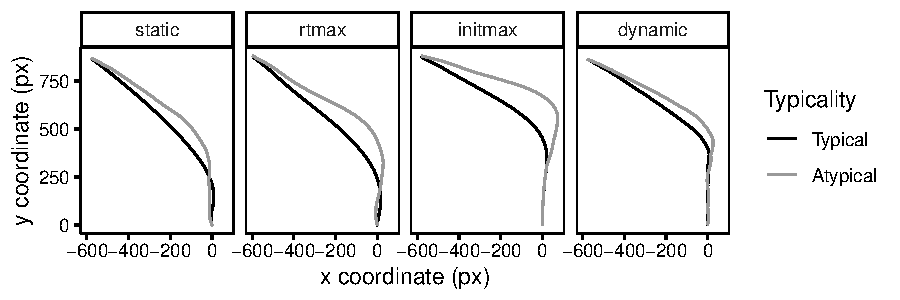
\includegraphics[keepaspectratio]{Duplicate-code_files/figure-latex/unnamed-chunk-25-1.pdf}}

\subsection{比较 MAD 指标}\label{ux6bd4ux8f83-mad-ux6307ux6807}

\subsubsection{每位参与者聚合 MAD
数据}\label{ux6bcfux4f4dux53c2ux4e0eux8005ux805aux5408-mad-ux6570ux636e}

\begin{Shaded}
\begin{Highlighting}[]
\CommentTok{\# 按 group 和 Typicality 聚合 MAD 指标,用于分析轨迹弯曲度的差异。}
\NormalTok{agg\_mad }\OtherTok{\textless{}{-}} \FunctionTok{mt\_aggregate\_per\_subject}\NormalTok{(mt\_data, }\AttributeTok{subject\_id =} \StringTok{"subject\_nr"}\NormalTok{,}
  \AttributeTok{use\_variables =} \StringTok{"MAD"}\NormalTok{, }\AttributeTok{use2\_variables =} \FunctionTok{c}\NormalTok{(}\StringTok{"Typicality"}\NormalTok{,}\StringTok{"group"}\NormalTok{))}
\end{Highlighting}
\end{Shaded}

\subsubsection{Descriptive 和 配对 t
检验}\label{descriptive-ux548c-ux914dux5bf9-t-ux68c0ux9a8c}

\begin{Shaded}
\begin{Highlighting}[]
\NormalTok{mad\_table }\OtherTok{\textless{}{-}}\NormalTok{ agg\_mad }\SpecialCharTok{\%\textgreater{}\%}
  \FunctionTok{group\_by}\NormalTok{(group) }\SpecialCharTok{\%\textgreater{}\%}
  \FunctionTok{select}\NormalTok{(MAD,group,Typicality) }\SpecialCharTok{\%\textgreater{}\%}
  \FunctionTok{summarize}\NormalTok{(}
    \AttributeTok{N =}  \FunctionTok{length}\NormalTok{(MAD[Typicality}\SpecialCharTok{==}\StringTok{"Typical"}\NormalTok{]),                     }\CommentTok{\# 典型条件下的样本数量}
    \AttributeTok{M\_t =} \FunctionTok{mean}\NormalTok{(MAD[Typicality}\SpecialCharTok{==}\StringTok{"Typical"}\NormalTok{]),                      }\CommentTok{\# 典型条件下 MAD 的平均值}
    \AttributeTok{SD\_t =} \FunctionTok{sd}\NormalTok{(MAD[Typicality}\SpecialCharTok{==}\StringTok{"Typical"}\NormalTok{]),                       }\CommentTok{\# 典型条件下 MAD 的标准差}
    \AttributeTok{M\_a =} \FunctionTok{mean}\NormalTok{(MAD[Typicality}\SpecialCharTok{==}\StringTok{"Atypical"}\NormalTok{]),                     }\CommentTok{\# 非典型条件下 MAD 的平均值}
    \AttributeTok{SD\_a =} \FunctionTok{sd}\NormalTok{(MAD[Typicality}\SpecialCharTok{==}\StringTok{"Atypical"}\NormalTok{]),                      }\CommentTok{\# 非典型条件下 MAD 的标准差}
    \AttributeTok{t =} \FunctionTok{t.test}\NormalTok{(MAD[Typicality}\SpecialCharTok{==}\StringTok{"Atypical"}\NormalTok{],MAD[Typicality}\SpecialCharTok{==}\StringTok{"Typical"}\NormalTok{],}\AttributeTok{paired=}\ConstantTok{TRUE}\NormalTok{)}\SpecialCharTok{$}\NormalTok{statistic, }\CommentTok{\# 配对样本 t 检验的 t 值}
    \AttributeTok{p =} \FunctionTok{t.test}\NormalTok{(MAD[Typicality}\SpecialCharTok{==}\StringTok{"Atypical"}\NormalTok{],MAD[Typicality}\SpecialCharTok{==}\StringTok{"Typical"}\NormalTok{],}\AttributeTok{paired=}\ConstantTok{TRUE}\NormalTok{)}\SpecialCharTok{$}\NormalTok{p.value,   }\CommentTok{\# 配对样本 t 检验的 p 值}
    \AttributeTok{d =}\NormalTok{ (M\_a}\SpecialCharTok{{-}}\NormalTok{M\_t)}\SpecialCharTok{/}\FunctionTok{sd}\NormalTok{(MAD[Typicality}\SpecialCharTok{==}\StringTok{"Atypical"}\NormalTok{]}\SpecialCharTok{{-}}\NormalTok{MAD[Typicality}\SpecialCharTok{==}\StringTok{"Typical"}\NormalTok{])                }\CommentTok{\# 效应量 Cohen\textquotesingle{}s d}
\NormalTok{    )}

\NormalTok{mad\_table }\SpecialCharTok{\%\textgreater{}\%}
  \FunctionTok{as.data.frame}\NormalTok{() }\SpecialCharTok{\%\textgreater{}\%}
  \FunctionTok{print}\NormalTok{(}\AttributeTok{digits=}\DecValTok{3}\NormalTok{)}
\end{Highlighting}
\end{Shaded}

\begin{verbatim}
##     group  N M_t SD_t M_a SD_a    t        p     d
## 1  static 59 185  134 270  173 4.18 1.01e-04 0.544
## 2   rtmax 60 190  151 301  198 4.32 6.00e-05 0.558
## 3 initmax 66 305  141 471  203 7.39 3.50e-10 0.910
## 4 dynamic 60 297  112 364  154 3.95 2.09e-04 0.510
\end{verbatim}

\subsubsection{图表}\label{ux56feux8868}

\begin{Shaded}
\begin{Highlighting}[]
\FunctionTok{ggplot}\NormalTok{(agg\_mad,}\FunctionTok{aes}\NormalTok{(}\AttributeTok{x=}\NormalTok{Typicality,}\AttributeTok{y=}\NormalTok{MAD,}\AttributeTok{linetype=}\NormalTok{group,}\AttributeTok{group=}\NormalTok{group))}\SpecialCharTok{+}
  \FunctionTok{geom\_line}\NormalTok{(}\AttributeTok{stat=}\StringTok{"summary"}\NormalTok{,}\AttributeTok{fun.y=}\StringTok{"mean"}\NormalTok{)}\SpecialCharTok{+}                    \CommentTok{\# 绘制平均值的折线图}
  \FunctionTok{geom\_point}\NormalTok{(}\AttributeTok{stat=}\StringTok{"summary"}\NormalTok{,}\AttributeTok{fun.y=}\StringTok{"mean"}\NormalTok{)}\SpecialCharTok{+}                   \CommentTok{\# 绘制平均值的点}
  \FunctionTok{geom\_errorbar}\NormalTok{(}\AttributeTok{stat=}\StringTok{"summary"}\NormalTok{,}\AttributeTok{fun.data=}\StringTok{"mean\_se"}\NormalTok{,}\AttributeTok{width=}\NormalTok{.}\DecValTok{2}\NormalTok{,}\AttributeTok{linetype=}\DecValTok{1}\NormalTok{)}\SpecialCharTok{+}  \CommentTok{\# 添加误差条(标准误)}
  \FunctionTok{scale\_linetype\_manual}\NormalTok{(}\AttributeTok{values=}\FunctionTok{c}\NormalTok{(}\DecValTok{1}\NormalTok{,}\DecValTok{2}\NormalTok{,}\DecValTok{3}\NormalTok{,}\DecValTok{4}\NormalTok{))}\SpecialCharTok{+}                    \CommentTok{\# 手动设置线型样式}
  \FunctionTok{coord\_cartesian}\NormalTok{(}\AttributeTok{ylim=}\FunctionTok{c}\NormalTok{(}\DecValTok{0}\NormalTok{,}\DecValTok{700}\NormalTok{))                              }\CommentTok{\# 设置 y 轴范围}
\end{Highlighting}
\end{Shaded}

\begin{verbatim}
## No summary function supplied, defaulting to `mean_se()`
## No summary function supplied, defaulting to `mean_se()`
\end{verbatim}

\pandocbounded{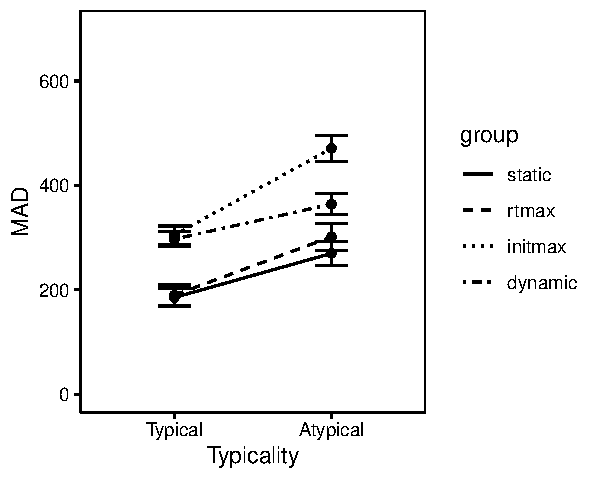
\includegraphics[keepaspectratio]{Duplicate-code_files/figure-latex/unnamed-chunk-28-1.pdf}}

\subsubsection{方差分析 ANOVA}\label{ux65b9ux5deeux5206ux6790-anova}

\begin{Shaded}
\begin{Highlighting}[]
\NormalTok{anova\_mad }\OtherTok{\textless{}{-}} \FunctionTok{aov\_ez}\NormalTok{(}\AttributeTok{data=}\NormalTok{agg\_mad, }\AttributeTok{dv =} \StringTok{"MAD"}\NormalTok{, }\AttributeTok{between =} \StringTok{"group"}\NormalTok{, }\AttributeTok{within =} \StringTok{"Typicality"}\NormalTok{,}
                    \AttributeTok{id =} \StringTok{"subject\_nr"}\NormalTok{)}
\end{Highlighting}
\end{Shaded}

\begin{verbatim}
## Contrasts set to contr.sum for the following variables: group
\end{verbatim}

\begin{Shaded}
\begin{Highlighting}[]
\FunctionTok{nice}\NormalTok{(anova\_mad,}\AttributeTok{es =} \FunctionTok{c}\NormalTok{(}\StringTok{"pes"}\NormalTok{,}\StringTok{"ges"}\NormalTok{))                          }\CommentTok{\# 显示 ANOVA 结果和效应量(部分 eta 平方、广义 eta 平方)}
\end{Highlighting}
\end{Shaded}

\begin{verbatim}
## Anova Table (Type 3 tests)
## 
## Response: MAD
##             Effect     df      MSE         F  ges  pes p.value
## 1            group 3, 241 37593.62 18.67 *** .144 .189   <.001
## 2       Typicality 1, 241 14412.64 97.72 *** .101 .289   <.001
## 3 group:Typicality 3, 241 14412.64   4.12 ** .014 .049    .007
## ---
## Signif. codes:  0 '***' 0.001 '**' 0.01 '*' 0.05 '+' 0.1 ' ' 1
\end{verbatim}

\begin{Shaded}
\begin{Highlighting}[]
\CommentTok{\# 计算部分 eta 平方的 90\% 置信区间}
\FunctionTok{round}\NormalTok{(}\FunctionTok{get\_partial\_etas}\NormalTok{(anova\_mad}\SpecialCharTok{$}\NormalTok{anova\_table, }\AttributeTok{conf.level=}\NormalTok{.}\DecValTok{90}\NormalTok{),}\DecValTok{2}\NormalTok{)}
\end{Highlighting}
\end{Shaded}

\begin{verbatim}
##                   pes lower upper
## group            0.19  0.11  0.25
## Typicality       0.29  0.21  0.36
## group:Typicality 0.05  0.01  0.09
\end{verbatim}

\subsection{对比分析}\label{ux5bf9ux6bd4ux5206ux6790}

\begin{Shaded}
\begin{Highlighting}[]
\CommentTok{\# 获取估计边际均值的组合}
\NormalTok{anova\_mad\_grid }\OtherTok{\textless{}{-}} \FunctionTok{lsmeans}\NormalTok{(anova\_mad,}\SpecialCharTok{\textasciitilde{}}\NormalTok{Typicality}\SpecialCharTok{:}\NormalTok{group)}

\CommentTok{\# 指定对比矩阵}
\NormalTok{contrast\_matrix\_complete }\OtherTok{\textless{}{-}} \FunctionTok{list}\NormalTok{(}
  \AttributeTok{typicality\_static =} \FunctionTok{c}\NormalTok{(}\SpecialCharTok{{-}}\DecValTok{1}\NormalTok{,}\DecValTok{1}\NormalTok{,}\DecValTok{0}\NormalTok{,}\DecValTok{0}\NormalTok{,}\DecValTok{0}\NormalTok{,}\DecValTok{0}\NormalTok{,}\DecValTok{0}\NormalTok{,}\DecValTok{0}\NormalTok{),                    }\CommentTok{\# 静态条件下典型性主效应}
  \AttributeTok{rtmax\_static\_main=}  \FunctionTok{c}\NormalTok{(}\SpecialCharTok{{-}}\DecValTok{1}\NormalTok{,}\SpecialCharTok{{-}}\DecValTok{1}\NormalTok{,}\DecValTok{1}\NormalTok{,}\DecValTok{1}\NormalTok{,}\DecValTok{0}\NormalTok{,}\DecValTok{0}\NormalTok{,}\DecValTok{0}\NormalTok{,}\DecValTok{0}\NormalTok{)}\SpecialCharTok{/}\DecValTok{2}\NormalTok{,                 }\CommentTok{\# RTmax vs 静态 的主效应}
  \AttributeTok{initmax\_static\_main =} \FunctionTok{c}\NormalTok{(}\SpecialCharTok{{-}}\DecValTok{1}\NormalTok{,}\SpecialCharTok{{-}}\DecValTok{1}\NormalTok{,}\DecValTok{0}\NormalTok{,}\DecValTok{0}\NormalTok{,}\DecValTok{1}\NormalTok{,}\DecValTok{1}\NormalTok{,}\DecValTok{0}\NormalTok{,}\DecValTok{0}\NormalTok{)}\SpecialCharTok{/}\DecValTok{2}\NormalTok{,               }\CommentTok{\# Initmax vs 静态 的主效应}
  \AttributeTok{dynamic\_static\_main =} \FunctionTok{c}\NormalTok{(}\SpecialCharTok{{-}}\DecValTok{1}\NormalTok{,}\SpecialCharTok{{-}}\DecValTok{1}\NormalTok{,}\DecValTok{0}\NormalTok{,}\DecValTok{0}\NormalTok{,}\DecValTok{0}\NormalTok{,}\DecValTok{0}\NormalTok{,}\DecValTok{1}\NormalTok{,}\DecValTok{1}\NormalTok{)}\SpecialCharTok{/}\DecValTok{2}\NormalTok{,               }\CommentTok{\# 动态 vs 静态 的主效应}
  \AttributeTok{rtmax\_static\_int =} \FunctionTok{c}\NormalTok{(}\DecValTok{1}\NormalTok{,}\SpecialCharTok{{-}}\DecValTok{1}\NormalTok{,}\SpecialCharTok{{-}}\DecValTok{1}\NormalTok{,}\DecValTok{1}\NormalTok{,}\DecValTok{0}\NormalTok{,}\DecValTok{0}\NormalTok{,}\DecValTok{0}\NormalTok{,}\DecValTok{0}\NormalTok{),                    }\CommentTok{\# RTmax vs 静态 的交互效应}
  \AttributeTok{initmax\_static\_int =} \FunctionTok{c}\NormalTok{(}\DecValTok{1}\NormalTok{,}\SpecialCharTok{{-}}\DecValTok{1}\NormalTok{,}\DecValTok{0}\NormalTok{,}\DecValTok{0}\NormalTok{,}\SpecialCharTok{{-}}\DecValTok{1}\NormalTok{,}\DecValTok{1}\NormalTok{,}\DecValTok{0}\NormalTok{,}\DecValTok{0}\NormalTok{),                  }\CommentTok{\# Initmax vs 静态 的交互效应}
  \AttributeTok{dynamic\_static\_int =} \FunctionTok{c}\NormalTok{(}\DecValTok{1}\NormalTok{,}\SpecialCharTok{{-}}\DecValTok{1}\NormalTok{,}\DecValTok{0}\NormalTok{,}\DecValTok{0}\NormalTok{,}\DecValTok{0}\NormalTok{,}\DecValTok{0}\NormalTok{,}\SpecialCharTok{{-}}\DecValTok{1}\NormalTok{,}\DecValTok{1}\NormalTok{))                  }\CommentTok{\# 动态 vs 静态 的交互效应}

\CommentTok{\# 进行对比检验}
\FunctionTok{contrast}\NormalTok{(anova\_mad\_grid,contrast\_matrix\_complete)}
\end{Highlighting}
\end{Shaded}

\begin{verbatim}
##  contrast            estimate   SE  df t.ratio p.value
##  typicality_static       84.5 22.1 241   3.822  0.0002
##  rtmax_static_main       18.2 25.1 241   0.723  0.4702
##  initmax_static_main    160.4 24.6 241   6.529  <.0001
##  dynamic_static_main    103.1 25.1 241   4.101  0.0001
##  rtmax_static_int        27.2 31.1 241   0.873  0.3833
##  initmax_static_int      81.6 30.4 241   2.684  0.0078
##  dynamic_static_int     -17.4 31.1 241  -0.560  0.5763
\end{verbatim}

\section{轨迹形状的分布}\label{ux8f68ux8ff9ux5f62ux72b6ux7684ux5206ux5e03}

\subsection{双峰系数(Bimodality
Coefficient)}\label{ux53ccux5cf0ux7cfbux6570bimodality-coefficient}

\begin{Shaded}
\begin{Highlighting}[]
\CommentTok{\# 按参与者标准化 MAD 值}
\NormalTok{mt\_data }\OtherTok{\textless{}{-}} \FunctionTok{mt\_standardize}\NormalTok{(mt\_data, }\AttributeTok{use\_variables =} \StringTok{"MAD"}\NormalTok{, }\AttributeTok{within =} \StringTok{"subject\_nr"}\NormalTok{)}

\CommentTok{\# 计算双峰系数}
\FunctionTok{mt\_check\_bimodality}\NormalTok{(mt\_data, }\AttributeTok{use\_variables =} \StringTok{"z\_MAD"}\NormalTok{,}
  \AttributeTok{grouping\_variables =} \FunctionTok{c}\NormalTok{(}\StringTok{"group"}\NormalTok{,}\StringTok{"Typicality"}\NormalTok{), }\AttributeTok{methods =} \StringTok{"BC"}\NormalTok{)}
\end{Highlighting}
\end{Shaded}

\begin{verbatim}
## $BC
##     group Typicality     z_MAD
## 1  static    Typical 0.5202425
## 2  static   Atypical 0.5479891
## 3   rtmax    Typical 0.5356378
## 4   rtmax   Atypical 0.5014132
## 5 initmax    Typical 0.5097199
## 6 initmax   Atypical 0.4731716
## 7 dynamic    Typical 0.5596031
## 8 dynamic   Atypical 0.5080918
\end{verbatim}

\subsection{平滑热图}\label{ux5e73ux6ed1ux70edux56fe}

\begin{Shaded}
\begin{Highlighting}[]
\NormalTok{heatmap\_smoothed }\OtherTok{\textless{}{-}} \FunctionTok{mt\_heatmap\_ggplot}\NormalTok{(mt\_data,}
  \AttributeTok{xres =} \DecValTok{1000}\NormalTok{,                       }\CommentTok{\# x 轴分辨率}
  \AttributeTok{smooth\_radius =} \DecValTok{20}\NormalTok{,               }\CommentTok{\# 平滑半径}
  \AttributeTok{n\_shades =} \DecValTok{10}\NormalTok{,                    }\CommentTok{\# 阴影层级}
  \AttributeTok{mean\_image =} \FloatTok{0.2}\NormalTok{,                 }\CommentTok{\# 平均图像透明度}
  \AttributeTok{colors=}\FunctionTok{c}\NormalTok{(}\StringTok{"white"}\NormalTok{,}\StringTok{"black"}\NormalTok{),        }\CommentTok{\# 使用黑白色调}
  \AttributeTok{facet\_col=}\StringTok{"group"}\NormalTok{)               }\CommentTok{\# 按组分面显示}
\end{Highlighting}
\end{Shaded}

\begin{verbatim}
## spatializing trajectories 
## calculate image 
## smooth image 
## enhance image by 4 
## spatializing trajectories 
## calculate image 
## smooth image 
## enhance image by 3.8 
## spatializing trajectories 
## calculate image 
## smooth image 
## enhance image by 3.7 
## spatializing trajectories 
## calculate image 
## smooth image 
## enhance image by 6.1
\end{verbatim}

\begin{Shaded}
\begin{Highlighting}[]
\NormalTok{heatmap\_smoothed}\SpecialCharTok{+}
  \FunctionTok{theme}\NormalTok{(}\AttributeTok{strip.background =} \FunctionTok{element\_rect}\NormalTok{(}\AttributeTok{colour =} \ConstantTok{NA}\NormalTok{))  }\CommentTok{\# 去除分面背景边框}
\end{Highlighting}
\end{Shaded}

\pandocbounded{\includegraphics[keepaspectratio]{Duplicate-code_files/figure-latex/unnamed-chunk-32-1.pdf}}

\subsection{原型分类(标准集合)}\label{ux539fux578bux5206ux7c7bux6807ux51c6ux96c6ux5408}

\subsubsection{绘制原型轨迹}\label{ux7ed8ux5236ux539fux578bux8f68ux8ff9}

\begin{Shaded}
\begin{Highlighting}[]
\FunctionTok{mt\_plot}\NormalTok{(mt\_prototypes,}\AttributeTok{facet\_col=}\StringTok{"mt\_id"}\NormalTok{,}\AttributeTok{only\_ggplot =} \ConstantTok{TRUE}\NormalTok{)}\SpecialCharTok{+}
  \FunctionTok{geom\_path}\NormalTok{()}\SpecialCharTok{+}
  \FunctionTok{facet\_grid}\NormalTok{(}\AttributeTok{cols =} \FunctionTok{vars}\NormalTok{(}\FunctionTok{factor}\NormalTok{(mt\_id,}\AttributeTok{levels=}\FunctionTok{rownames}\NormalTok{(mt\_prototypes))))}\SpecialCharTok{+}  \CommentTok{\# 自定义排列顺序}
  \FunctionTok{theme}\NormalTok{(}\AttributeTok{axis.text=}\NormalTok{ggplot2}\SpecialCharTok{::}\FunctionTok{element\_blank}\NormalTok{(),}\AttributeTok{axis.ticks=}\NormalTok{ggplot2}\SpecialCharTok{::}\FunctionTok{element\_blank}\NormalTok{())  }\CommentTok{\# 隐藏坐标轴文本与刻度}
\end{Highlighting}
\end{Shaded}

\pandocbounded{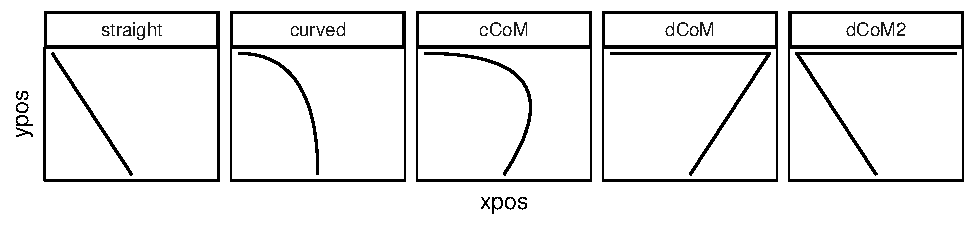
\includegraphics[keepaspectratio]{Duplicate-code_files/figure-latex/unnamed-chunk-33-1.pdf}}
\#\#\# 将轨迹映射到原型

\begin{Shaded}
\begin{Highlighting}[]
\NormalTok{mt\_data }\OtherTok{\textless{}{-}} \FunctionTok{mt\_spatialize}\NormalTok{(mt\_data)}
\NormalTok{mt\_data }\OtherTok{\textless{}{-}} \FunctionTok{mt\_map}\NormalTok{(mt\_data,}\AttributeTok{prototypes =}\NormalTok{ mt\_prototypes,}
  \AttributeTok{save\_as =} \StringTok{"measures"}\NormalTok{, }\AttributeTok{grouping\_variables =} \StringTok{"group"}\NormalTok{)}
\NormalTok{mt\_data}\SpecialCharTok{$}\NormalTok{data}\SpecialCharTok{$}\NormalTok{prototype\_label }\OtherTok{\textless{}{-}}\NormalTok{ mt\_data}\SpecialCharTok{$}\NormalTok{measures}\SpecialCharTok{$}\NormalTok{prototype\_label}
\end{Highlighting}
\end{Shaded}

\subsubsection{每组的轨迹分类}\label{ux6bcfux7ec4ux7684ux8f68ux8ff9ux5206ux7c7b}

\paragraph{相对频率}\label{ux76f8ux5bf9ux9891ux7387}

\begin{Shaded}
\begin{Highlighting}[]
\NormalTok{prototype\_percentages }\OtherTok{\textless{}{-}}\NormalTok{ mt\_data}\SpecialCharTok{$}\NormalTok{data }\SpecialCharTok{\%\textgreater{}\%}
  \FunctionTok{group\_by}\NormalTok{(group,prototype\_label) }\SpecialCharTok{\%\textgreater{}\%}
  \FunctionTok{summarise}\NormalTok{(}\AttributeTok{n=}\FunctionTok{n}\NormalTok{()) }\SpecialCharTok{\%\textgreater{}\%}
  \FunctionTok{mutate}\NormalTok{(}\AttributeTok{Percent=}\FunctionTok{paste}\NormalTok{(}\FunctionTok{round}\NormalTok{(}\DecValTok{100}\SpecialCharTok{*}\NormalTok{n}\SpecialCharTok{/}\FunctionTok{sum}\NormalTok{(n)),}\StringTok{"\%"}\NormalTok{,}\AttributeTok{sep=}\StringTok{""}\NormalTok{))}
\end{Highlighting}
\end{Shaded}

\begin{verbatim}
## `summarise()` has grouped output by 'group'. You can override using the
## `.groups` argument.
\end{verbatim}

\begin{Shaded}
\begin{Highlighting}[]
\FunctionTok{mt\_plot}\NormalTok{(mt\_data, }\AttributeTok{use =} \StringTok{"sp\_trajectories"}\NormalTok{,}
  \AttributeTok{x =} \StringTok{"xpos"}\NormalTok{, }\AttributeTok{y =} \StringTok{"ypos"}\NormalTok{, }\AttributeTok{facet\_col =} \StringTok{"prototype\_label"}\NormalTok{, }\AttributeTok{facet\_row=}\StringTok{"group"}\NormalTok{,}\AttributeTok{alpha=}\NormalTok{.}\DecValTok{2}\NormalTok{)}\SpecialCharTok{+}
  \FunctionTok{xlab}\NormalTok{(}\StringTok{"x 坐标 (px)"}\NormalTok{) }\SpecialCharTok{+} \FunctionTok{ylab}\NormalTok{(}\StringTok{"y 坐标 (px)"}\NormalTok{)}\SpecialCharTok{+} 
  \FunctionTok{geom\_text}\NormalTok{(}\AttributeTok{data=}\NormalTok{prototype\_percentages,}\FunctionTok{aes}\NormalTok{(}\AttributeTok{label=}\NormalTok{Percent),}\AttributeTok{x=}\DecValTok{650}\NormalTok{,}\AttributeTok{y=}\DecValTok{50}\NormalTok{)}\SpecialCharTok{+}
  \FunctionTok{scale\_y\_continuous}\NormalTok{(}\AttributeTok{breaks=}\FunctionTok{c}\NormalTok{(}\DecValTok{0}\NormalTok{,}\DecValTok{500}\NormalTok{,}\DecValTok{1000}\NormalTok{))}\SpecialCharTok{+} 
  \FunctionTok{coord\_cartesian}\NormalTok{(}\AttributeTok{xlim=}\FunctionTok{c}\NormalTok{(}\SpecialCharTok{{-}}\DecValTok{900}\NormalTok{,}\DecValTok{900}\NormalTok{))}
\end{Highlighting}
\end{Shaded}

\pandocbounded{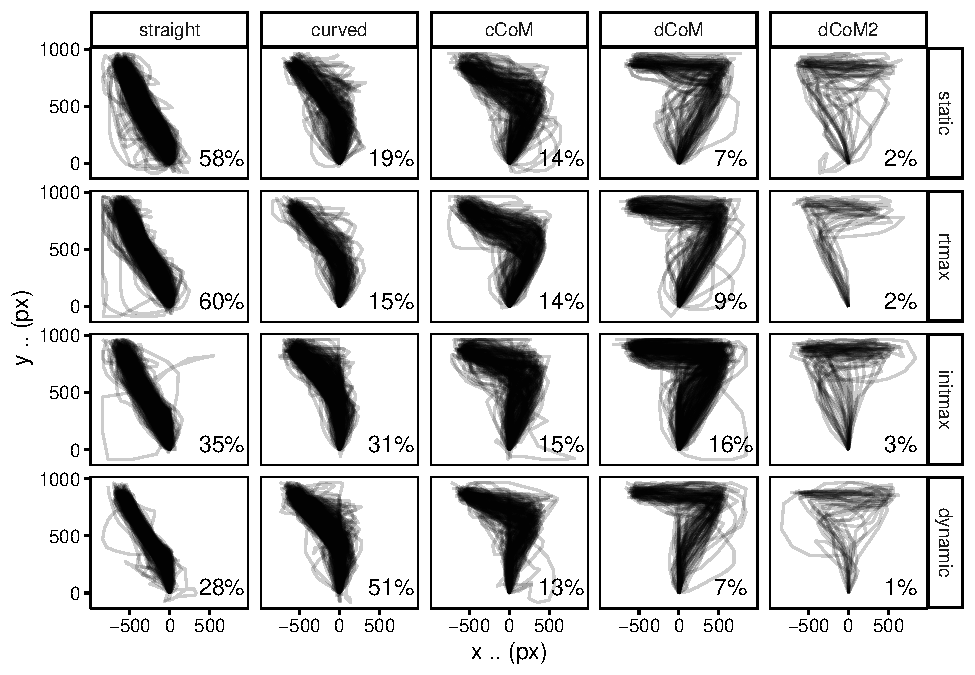
\includegraphics[keepaspectratio]{Duplicate-code_files/figure-latex/unnamed-chunk-35-1.pdf}}

\paragraph{卡方检验}\label{ux5361ux65b9ux68c0ux9a8c-1}

\begin{Shaded}
\begin{Highlighting}[]
\FunctionTok{chisq.test}\NormalTok{(}\FunctionTok{with}\NormalTok{(mt\_data}\SpecialCharTok{$}\NormalTok{data,}\FunctionTok{table}\NormalTok{(group, prototype\_label)))}
\end{Highlighting}
\end{Shaded}

\begin{verbatim}
## 
##  Pearson's Chi-squared test
## 
## data:  with(mt_data$data, table(group, prototype_label))
## X-squared = 535.73, df = 12, p-value < 2.2e-16
\end{verbatim}

\subsubsection{每组 X
典型性条件的轨迹分类}\label{ux6bcfux7ec4-x-ux5178ux578bux6027ux6761ux4ef6ux7684ux8f68ux8ff9ux5206ux7c7b}

\paragraph{相对频率}\label{ux76f8ux5bf9ux9891ux7387-1}

\begin{Shaded}
\begin{Highlighting}[]
\NormalTok{rel\_freq\_agg }\OtherTok{\textless{}{-}}\NormalTok{ mt\_data}\SpecialCharTok{$}\NormalTok{data }\SpecialCharTok{\%\textgreater{}\%}
  \FunctionTok{group\_by}\NormalTok{(group,Typicality,prototype\_label) }\SpecialCharTok{\%\textgreater{}\%}
  \FunctionTok{summarise}\NormalTok{(}\AttributeTok{n=}\FunctionTok{n}\NormalTok{()) }\SpecialCharTok{\%\textgreater{}\%}
  \FunctionTok{mutate}\NormalTok{(}\AttributeTok{Percent=}\NormalTok{n}\SpecialCharTok{/}\FunctionTok{sum}\NormalTok{(n))}
\end{Highlighting}
\end{Shaded}

\begin{verbatim}
## `summarise()` has grouped output by 'group', 'Typicality'. You can override
## using the `.groups` argument.
\end{verbatim}

\begin{Shaded}
\begin{Highlighting}[]
\FunctionTok{spread}\NormalTok{(rel\_freq\_agg[,}\SpecialCharTok{{-}}\DecValTok{4}\NormalTok{],}\StringTok{"prototype\_label"}\NormalTok{,}\StringTok{"Percent"}\NormalTok{,}\AttributeTok{fill =} \DecValTok{0}\NormalTok{) }\SpecialCharTok{\%\textgreater{}\%}
  \FunctionTok{as.data.frame}\NormalTok{()}\SpecialCharTok{\%\textgreater{}\%}
  \FunctionTok{print}\NormalTok{(}\AttributeTok{digits=}\DecValTok{2}\NormalTok{)}
\end{Highlighting}
\end{Shaded}

\begin{verbatim}
##     group Typicality straight curved cCoM  dCoM  dCoM2
## 1  static    Typical     0.62   0.19 0.12 0.054 0.0163
## 2  static   Atypical     0.49   0.20 0.18 0.098 0.0379
## 3   rtmax    Typical     0.64   0.15 0.13 0.069 0.0096
## 4   rtmax   Atypical     0.50   0.15 0.18 0.139 0.0314
## 5 initmax    Typical     0.39   0.33 0.14 0.119 0.0163
## 6 initmax   Atypical     0.24   0.27 0.17 0.264 0.0578
## 7 dynamic    Typical     0.28   0.53 0.13 0.057 0.0053
## 8 dynamic   Atypical     0.26   0.45 0.15 0.098 0.0379
\end{verbatim}

\begin{Shaded}
\begin{Highlighting}[]
\FunctionTok{ggplot}\NormalTok{(rel\_freq\_agg,}\FunctionTok{aes}\NormalTok{(}\AttributeTok{x=}\NormalTok{Typicality,}\AttributeTok{y=}\NormalTok{Percent,}\AttributeTok{fill=}\NormalTok{forcats}\SpecialCharTok{::}\FunctionTok{fct\_rev}\NormalTok{(prototype\_label)))}\SpecialCharTok{+}
  \FunctionTok{geom\_bar}\NormalTok{(}\AttributeTok{stat=}\StringTok{"identity"}\NormalTok{,}\AttributeTok{color=}\StringTok{"black"}\NormalTok{)}\SpecialCharTok{+}
  \FunctionTok{scale\_fill\_brewer}\NormalTok{(}\AttributeTok{type=}\StringTok{"seq"}\NormalTok{,}\AttributeTok{name=}\StringTok{"分类"}\NormalTok{)}\SpecialCharTok{+}
  \FunctionTok{facet\_grid}\NormalTok{(.}\SpecialCharTok{\textasciitilde{}}\NormalTok{group)}
\end{Highlighting}
\end{Shaded}

\pandocbounded{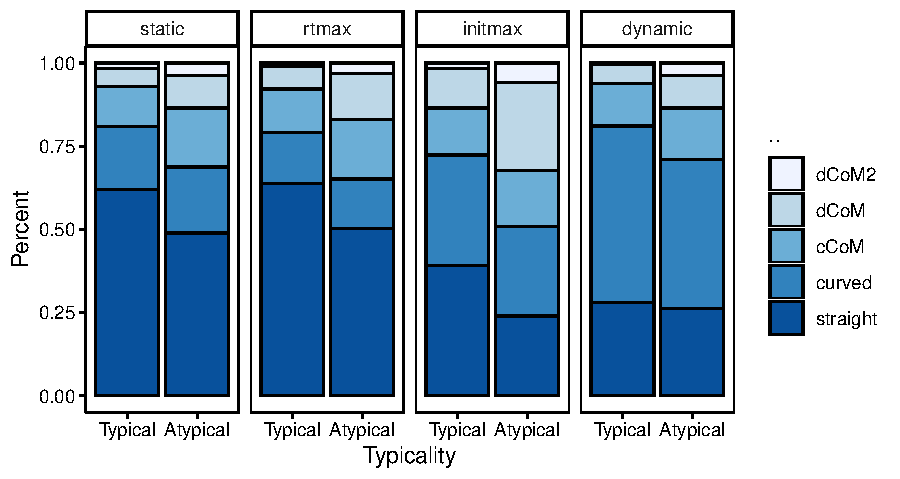
\includegraphics[keepaspectratio]{Duplicate-code_files/figure-latex/unnamed-chunk-37-1.pdf}}

\paragraph{有序混合回归}\label{ux6709ux5e8fux6df7ux5408ux56deux5f52}

\begin{Shaded}
\begin{Highlighting}[]
\FunctionTok{contrasts}\NormalTok{(mt\_data}\SpecialCharTok{$}\NormalTok{data}\SpecialCharTok{$}\NormalTok{Typicality) }\OtherTok{\textless{}{-}} \FunctionTok{c}\NormalTok{(}\SpecialCharTok{{-}}\FloatTok{0.5}\NormalTok{,}\FloatTok{0.5}\NormalTok{)}
\CommentTok{\# 对 group 使用默认对比(以 static 为基线的虚拟编码)}
\FunctionTok{contrasts}\NormalTok{(mt\_data}\SpecialCharTok{$}\NormalTok{data}\SpecialCharTok{$}\NormalTok{group)}
\end{Highlighting}
\end{Shaded}

\begin{verbatim}
##         rtmax initmax dynamic
## static      0       0       0
## rtmax       1       0       0
## initmax     0       1       0
## dynamic     0       0       1
\end{verbatim}

\begin{Shaded}
\begin{Highlighting}[]
\FunctionTok{summary}\NormalTok{(}\FunctionTok{clmm}\NormalTok{(prototype\_label}\SpecialCharTok{\textasciitilde{}}\NormalTok{Typicality}\SpecialCharTok{*}\NormalTok{group}\SpecialCharTok{+}\NormalTok{(}\DecValTok{1}\SpecialCharTok{|}\NormalTok{subject\_nr),}\AttributeTok{data=}\NormalTok{mt\_data}\SpecialCharTok{$}\NormalTok{data))}
\end{Highlighting}
\end{Shaded}

\begin{verbatim}
## Cumulative Link Mixed Model fitted with the Laplace approximation
## 
## formula: prototype_label ~ Typicality * group + (1 | subject_nr)
## data:    mt_data$data
## 
##  link  threshold nobs logLik   AIC      niter      max.grad cond.H 
##  logit flexible  4263 -5228.98 10481.96 1420(5684) 4.99e-03 2.4e+02
## 
## Random effects:
##  Groups     Name        Variance Std.Dev.
##  subject_nr (Intercept) 0.6917   0.8317  
## Number of groups:  subject_nr 245 
## 
## Coefficients:
##                          Estimate Std. Error z value Pr(>|z|)    
## Typicality1               0.69431    0.13716   5.062 4.15e-07 ***
## grouprtmax                0.05605    0.18342   0.306   0.7599    
## groupinitmax              1.05662    0.17657   5.984 2.18e-09 ***
## groupdynamic              0.77965    0.17838   4.371 1.24e-05 ***
## Typicality1:grouprtmax    0.15934    0.20078   0.794   0.4274    
## Typicality1:groupinitmax  0.30873    0.18414   1.677   0.0936 .  
## Typicality1:groupdynamic -0.39681    0.18115  -2.191   0.0285 *  
## ---
## Signif. codes:  0 '***' 0.001 '**' 0.01 '*' 0.05 '.' 0.1 ' ' 1
## 
## Threshold coefficients:
##                 Estimate Std. Error z value
## straight|curved   0.1227     0.1296   0.946
## curved|cCoM       1.6248     0.1323  12.283
## cCoM|dCoM         2.6964     0.1371  19.667
## dCoM|dCoM2        4.6552     0.1693  27.504
\end{verbatim}

\subsection{原型分类(扩展原型集)}\label{ux539fux578bux5206ux7c7bux6269ux5c55ux539fux578bux96c6}

\subsubsection{扩展原型集}\label{ux6269ux5c55ux539fux578bux96c6}

包含轨迹先向上移动到屏幕顶部然后\ldots{} * 向左到达被选选项(upleft) *
向右到未被选选项然后再向左(upCoM) *
向左到被选项,然后向右到未被选项,再向左一次(upCoM2)

\begin{Shaded}
\begin{Highlighting}[]
\NormalTok{mt\_prototypes\_ext }\OtherTok{\textless{}{-}} \FunctionTok{mt\_add\_trajectory}\NormalTok{(mt\_prototypes,}
   \AttributeTok{xpos =} \FunctionTok{c}\NormalTok{(}\DecValTok{0}\NormalTok{,}\DecValTok{0}\NormalTok{,}\SpecialCharTok{{-}}\DecValTok{1}\NormalTok{), }\AttributeTok{ypos =} \FunctionTok{c}\NormalTok{(}\DecValTok{0}\NormalTok{,}\FloatTok{1.5}\NormalTok{,}\FloatTok{1.5}\NormalTok{), }\AttributeTok{id =} \StringTok{"upleft"}
\NormalTok{)}

\NormalTok{mt\_prototypes\_ext }\OtherTok{\textless{}{-}} \FunctionTok{mt\_add\_trajectory}\NormalTok{(mt\_prototypes\_ext,}
   \AttributeTok{xpos =} \FunctionTok{c}\NormalTok{(}\DecValTok{0}\NormalTok{,}\DecValTok{0}\NormalTok{,}\DecValTok{1}\NormalTok{,}\SpecialCharTok{{-}}\DecValTok{1}\NormalTok{), }\AttributeTok{ypos =} \FunctionTok{c}\NormalTok{(}\DecValTok{0}\NormalTok{,}\FloatTok{1.5}\NormalTok{,}\FloatTok{1.5}\NormalTok{,}\FloatTok{1.5}\NormalTok{), }\AttributeTok{id =} \StringTok{"upCoM"}
\NormalTok{)}

\NormalTok{mt\_prototypes\_ext }\OtherTok{\textless{}{-}} \FunctionTok{mt\_add\_trajectory}\NormalTok{(mt\_prototypes\_ext,}
   \AttributeTok{xpos =} \FunctionTok{c}\NormalTok{(}\DecValTok{0}\NormalTok{,}\DecValTok{0}\NormalTok{,}\SpecialCharTok{{-}}\DecValTok{1}\NormalTok{,}\DecValTok{1}\NormalTok{,}\SpecialCharTok{{-}}\DecValTok{1}\NormalTok{), }\AttributeTok{ypos =} \FunctionTok{c}\NormalTok{(}\DecValTok{0}\NormalTok{,}\FloatTok{1.5}\NormalTok{,}\FloatTok{1.5}\NormalTok{,}\FloatTok{1.5}\NormalTok{,}\FloatTok{1.5}\NormalTok{), }\AttributeTok{id =} \StringTok{"upCoM2"}
\NormalTok{)}

\NormalTok{prototype\_labels\_extended }\OtherTok{\textless{}{-}} 
  \FunctionTok{c}\NormalTok{(}\StringTok{"straight"}\NormalTok{,}\StringTok{"curved"}\NormalTok{,}\StringTok{"upleft"}\NormalTok{,}\StringTok{"cCoM"}\NormalTok{,}\StringTok{"upCoM"}\NormalTok{,}\StringTok{"dCoM"}\NormalTok{,}\StringTok{"upCoM2"}\NormalTok{,}\StringTok{"dCoM2"}\NormalTok{)}

\FunctionTok{mt\_plot}\NormalTok{(mt\_prototypes\_ext,}\AttributeTok{facet\_col=}\StringTok{"mt\_id"}\NormalTok{,}\AttributeTok{only\_ggplot =} \ConstantTok{TRUE}\NormalTok{)}\SpecialCharTok{+}
  \FunctionTok{geom\_path}\NormalTok{()}\SpecialCharTok{+}
  \FunctionTok{facet\_grid}\NormalTok{(}\AttributeTok{cols =} \FunctionTok{vars}\NormalTok{(}\FunctionTok{factor}\NormalTok{(mt\_id,}\AttributeTok{levels=}\NormalTok{prototype\_labels\_extended)))}\SpecialCharTok{+}
  \FunctionTok{theme}\NormalTok{(}\AttributeTok{axis.text=}\NormalTok{ggplot2}\SpecialCharTok{::}\FunctionTok{element\_blank}\NormalTok{(),}\AttributeTok{axis.ticks=}\NormalTok{ggplot2}\SpecialCharTok{::}\FunctionTok{element\_blank}\NormalTok{()) }
\end{Highlighting}
\end{Shaded}

\pandocbounded{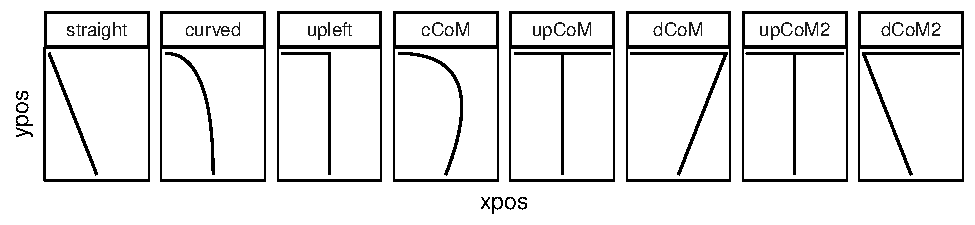
\includegraphics[keepaspectratio]{Duplicate-code_files/figure-latex/unnamed-chunk-39-1.pdf}}

\subsubsection{将轨迹映射到原型}\label{ux5c06ux8f68ux8ff9ux6620ux5c04ux5230ux539fux578b}

\begin{Shaded}
\begin{Highlighting}[]
\NormalTok{mt\_data }\OtherTok{\textless{}{-}} \FunctionTok{mt\_spatialize}\NormalTok{(mt\_data)}
\NormalTok{mt\_data }\OtherTok{\textless{}{-}} \FunctionTok{mt\_map}\NormalTok{(mt\_data,}\AttributeTok{prototypes =}\NormalTok{ mt\_prototypes\_ext,}
  \AttributeTok{save\_as=}\StringTok{"measures"}\NormalTok{, }\AttributeTok{grouping\_variables =} \StringTok{"group"}\NormalTok{)}

\CommentTok{\# 创建包含所有原型按升序排列的变量}
\NormalTok{mt\_data}\SpecialCharTok{$}\NormalTok{data}\SpecialCharTok{$}\NormalTok{prototype\_label }\OtherTok{\textless{}{-}} \FunctionTok{factor}\NormalTok{(mt\_data}\SpecialCharTok{$}\NormalTok{measures}\SpecialCharTok{$}\NormalTok{prototype\_label,}
  \AttributeTok{levels=}\NormalTok{prototype\_labels\_extended)}

\CommentTok{\# 创建变量,将“up”类型的原型归为其弯曲(curved)等价类别}
\NormalTok{mt\_data}\SpecialCharTok{$}\NormalTok{data}\SpecialCharTok{$}\NormalTok{prototype\_label\_red }\OtherTok{\textless{}{-}} \FunctionTok{factor}\NormalTok{(mt\_data}\SpecialCharTok{$}\NormalTok{measures}\SpecialCharTok{$}\NormalTok{prototype\_label,}
  \AttributeTok{levels=}\FunctionTok{c}\NormalTok{(}\StringTok{"straight"}\NormalTok{,}\StringTok{"curved"}\NormalTok{,}\StringTok{"upleft"}\NormalTok{,}\StringTok{"cCoM"}\NormalTok{,}\StringTok{"upCoM"}\NormalTok{,}\StringTok{"dCoM"}\NormalTok{,}\StringTok{"upCoM2"}\NormalTok{,}\StringTok{"dCoM2"}\NormalTok{),}
  \AttributeTok{labels=}\FunctionTok{c}\NormalTok{(}\StringTok{"straight"}\NormalTok{,}\StringTok{"curved"}\NormalTok{,}\StringTok{"curved"}\NormalTok{,}\StringTok{"cCoM"}\NormalTok{,}\StringTok{"cCoM"}\NormalTok{, }\StringTok{"dCoM"}\NormalTok{,}\StringTok{"dCoM2"}\NormalTok{, }\StringTok{"dCoM2"}\NormalTok{))}
\end{Highlighting}
\end{Shaded}

\subsubsection{每组的轨迹分类}\label{ux6bcfux7ec4ux7684ux8f68ux8ff9ux5206ux7c7b-1}

\paragraph{相对频率}\label{ux76f8ux5bf9ux9891ux7387-2}

\begin{Shaded}
\begin{Highlighting}[]
\NormalTok{prototype\_percentages }\OtherTok{\textless{}{-}}\NormalTok{ mt\_data}\SpecialCharTok{$}\NormalTok{data }\SpecialCharTok{\%\textgreater{}\%}
  \FunctionTok{group\_by}\NormalTok{(group,prototype\_label) }\SpecialCharTok{\%\textgreater{}\%}
  \FunctionTok{summarise}\NormalTok{(}\AttributeTok{n=}\FunctionTok{n}\NormalTok{()) }\SpecialCharTok{\%\textgreater{}\%}
  \FunctionTok{mutate}\NormalTok{(}\AttributeTok{Percent=}\FunctionTok{paste}\NormalTok{(}\FunctionTok{round}\NormalTok{(}\DecValTok{100}\SpecialCharTok{*}\NormalTok{n}\SpecialCharTok{/}\FunctionTok{sum}\NormalTok{(n)),}\StringTok{"\%"}\NormalTok{,}\AttributeTok{sep=}\StringTok{""}\NormalTok{))}
\end{Highlighting}
\end{Shaded}

\begin{verbatim}
## `summarise()` has grouped output by 'group'. You can override using the
## `.groups` argument.
\end{verbatim}

\begin{Shaded}
\begin{Highlighting}[]
\FunctionTok{mt\_plot}\NormalTok{(mt\_data, }\AttributeTok{use =} \StringTok{"sp\_trajectories"}\NormalTok{,}
  \AttributeTok{x =} \StringTok{"xpos"}\NormalTok{, }\AttributeTok{y =} \StringTok{"ypos"}\NormalTok{, }\AttributeTok{facet\_col =} \StringTok{"prototype\_label"}\NormalTok{, }\AttributeTok{facet\_row=}\StringTok{"group"}\NormalTok{,}\AttributeTok{alpha=}\NormalTok{.}\DecValTok{2}\NormalTok{)}\SpecialCharTok{+}
  \FunctionTok{xlab}\NormalTok{(}\StringTok{"x 坐标 (px)"}\NormalTok{) }\SpecialCharTok{+} \FunctionTok{ylab}\NormalTok{(}\StringTok{"y 坐标 (px)"}\NormalTok{)}\SpecialCharTok{+} 
  \FunctionTok{geom\_text}\NormalTok{(}\AttributeTok{data=}\NormalTok{prototype\_percentages,}\FunctionTok{aes}\NormalTok{(}\AttributeTok{label=}\NormalTok{Percent),}\AttributeTok{x=}\DecValTok{650}\NormalTok{,}\AttributeTok{y=}\DecValTok{50}\NormalTok{)}\SpecialCharTok{+}
  \FunctionTok{scale\_y\_continuous}\NormalTok{(}\AttributeTok{breaks=}\FunctionTok{c}\NormalTok{(}\DecValTok{0}\NormalTok{,}\DecValTok{500}\NormalTok{,}\DecValTok{1000}\NormalTok{))}\SpecialCharTok{+} 
  \FunctionTok{coord\_cartesian}\NormalTok{(}\AttributeTok{xlim=}\FunctionTok{c}\NormalTok{(}\SpecialCharTok{{-}}\DecValTok{900}\NormalTok{,}\DecValTok{900}\NormalTok{))}
\end{Highlighting}
\end{Shaded}

\pandocbounded{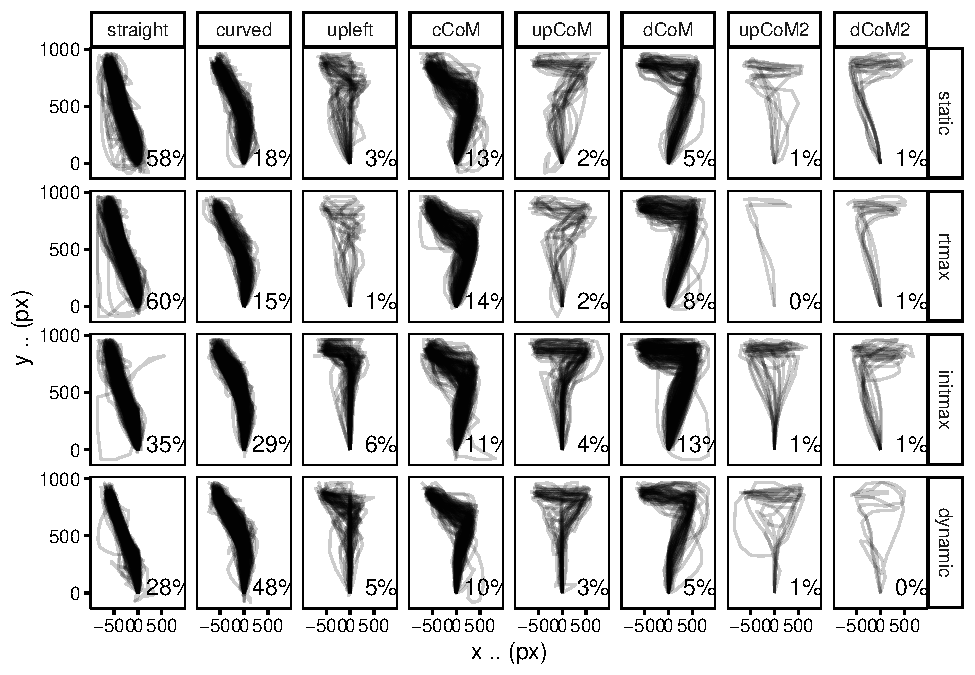
\includegraphics[keepaspectratio]{Duplicate-code_files/figure-latex/unnamed-chunk-41-1.pdf}}

\paragraph{卡方检验}\label{ux5361ux65b9ux68c0ux9a8c-2}

\begin{Shaded}
\begin{Highlighting}[]
\FunctionTok{chisq.test}\NormalTok{(}\FunctionTok{with}\NormalTok{(mt\_data}\SpecialCharTok{$}\NormalTok{data,}\FunctionTok{table}\NormalTok{(group, prototype\_label)))}
\end{Highlighting}
\end{Shaded}

\begin{verbatim}
## 
##  Pearson's Chi-squared test
## 
## data:  with(mt_data$data, table(group, prototype_label))
## X-squared = 580.8, df = 21, p-value < 2.2e-16
\end{verbatim}

\subsubsection{每组 X
典型性条件的轨迹分类}\label{ux6bcfux7ec4-x-ux5178ux578bux6027ux6761ux4ef6ux7684ux8f68ux8ff9ux5206ux7c7b-1}

\paragraph{相对频率}\label{ux76f8ux5bf9ux9891ux7387-3}

\begin{Shaded}
\begin{Highlighting}[]
\NormalTok{rel\_freq\_agg }\OtherTok{\textless{}{-}}\NormalTok{ mt\_data}\SpecialCharTok{$}\NormalTok{data }\SpecialCharTok{\%\textgreater{}\%}
  \FunctionTok{group\_by}\NormalTok{(group,Typicality,prototype\_label) }\SpecialCharTok{\%\textgreater{}\%}
  \FunctionTok{summarise}\NormalTok{(}\AttributeTok{n=}\FunctionTok{n}\NormalTok{()) }\SpecialCharTok{\%\textgreater{}\%}
  \FunctionTok{mutate}\NormalTok{(}\AttributeTok{Percent=}\NormalTok{n}\SpecialCharTok{/}\FunctionTok{sum}\NormalTok{(n), }\AttributeTok{Percent\_rounded =} \FunctionTok{round}\NormalTok{(Percent,}\DecValTok{2}\NormalTok{))}
\end{Highlighting}
\end{Shaded}

\begin{verbatim}
## `summarise()` has grouped output by 'group', 'Typicality'. You can override
## using the `.groups` argument.
\end{verbatim}

\begin{Shaded}
\begin{Highlighting}[]
\FunctionTok{spread}\NormalTok{(rel\_freq\_agg[,}\SpecialCharTok{{-}}\FunctionTok{c}\NormalTok{(}\DecValTok{4}\SpecialCharTok{:}\DecValTok{5}\NormalTok{)],}\StringTok{"prototype\_label"}\NormalTok{,}\StringTok{"Percent\_rounded"}\NormalTok{,}\AttributeTok{fill =} \DecValTok{0}\NormalTok{) }\SpecialCharTok{\%\textgreater{}\%}
  \FunctionTok{as.data.frame}\NormalTok{()}
\end{Highlighting}
\end{Shaded}

\begin{verbatim}
##     group Typicality straight curved upleft cCoM upCoM dCoM upCoM2 dCoM2
## 1  static    Typical     0.62   0.17   0.03 0.11  0.01 0.04   0.01  0.01
## 2  static   Atypical     0.49   0.18   0.04 0.16  0.03 0.07   0.01  0.02
## 3   rtmax    Typical     0.64   0.15   0.01 0.12  0.01 0.06   0.00  0.00
## 4   rtmax   Atypical     0.50   0.14   0.02 0.16  0.03 0.12   0.00  0.02
## 5 initmax    Typical     0.39   0.30   0.06 0.11  0.02 0.10   0.01  0.00
## 6 initmax   Atypical     0.24   0.24   0.06 0.13  0.09 0.19   0.03  0.03
## 7 dynamic    Typical     0.28   0.51   0.05 0.10  0.02 0.04   0.00  0.00
## 8 dynamic   Atypical     0.26   0.42   0.07 0.11  0.04 0.07   0.02  0.01
\end{verbatim}

\begin{Shaded}
\begin{Highlighting}[]
\FunctionTok{ggplot}\NormalTok{(rel\_freq\_agg,}\FunctionTok{aes}\NormalTok{(}\AttributeTok{x=}\NormalTok{Typicality,}\AttributeTok{y=}\NormalTok{Percent,}\AttributeTok{fill=}\NormalTok{forcats}\SpecialCharTok{::}\FunctionTok{fct\_rev}\NormalTok{(prototype\_label)))}\SpecialCharTok{+}
  \FunctionTok{geom\_bar}\NormalTok{(}\AttributeTok{stat=}\StringTok{"identity"}\NormalTok{,}\AttributeTok{color=}\StringTok{"black"}\NormalTok{)}\SpecialCharTok{+}
  \FunctionTok{scale\_fill\_brewer}\NormalTok{(}\AttributeTok{type=}\StringTok{"seq"}\NormalTok{,}\AttributeTok{name=}\StringTok{"分类"}\NormalTok{)}\SpecialCharTok{+}
  \FunctionTok{facet\_grid}\NormalTok{(.}\SpecialCharTok{\textasciitilde{}}\NormalTok{group)}
\end{Highlighting}
\end{Shaded}

\pandocbounded{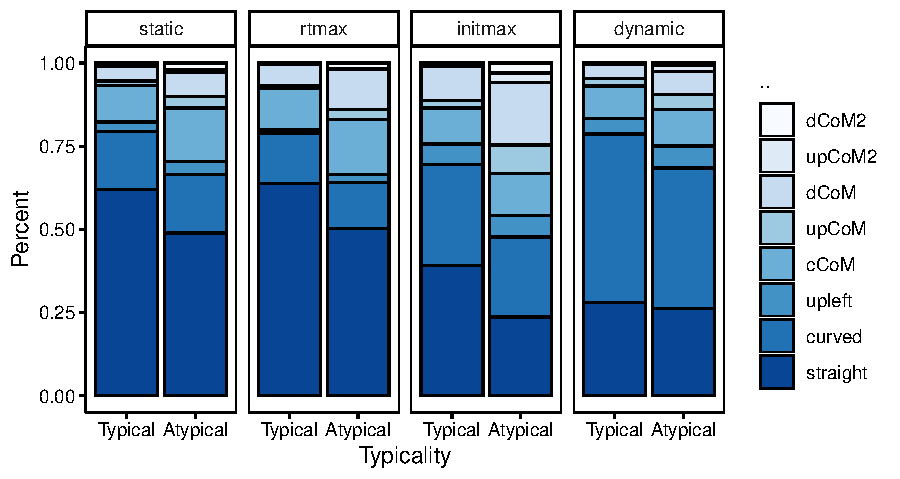
\includegraphics[keepaspectratio]{Duplicate-code_files/figure-latex/unnamed-chunk-43-1.pdf}}

\paragraph{有序混合回归(将所有原型视为有序)}\label{ux6709ux5e8fux6df7ux5408ux56deux5f52ux5c06ux6240ux6709ux539fux578bux89c6ux4e3aux6709ux5e8f}

\begin{Shaded}
\begin{Highlighting}[]
\FunctionTok{summary}\NormalTok{(}\FunctionTok{clmm}\NormalTok{(prototype\_label}\SpecialCharTok{\textasciitilde{}}\NormalTok{Typicality}\SpecialCharTok{*}\NormalTok{group}\SpecialCharTok{+}\NormalTok{(}\DecValTok{1}\SpecialCharTok{|}\NormalTok{subject\_nr),}\AttributeTok{data=}\NormalTok{mt\_data}\SpecialCharTok{$}\NormalTok{data))}
\end{Highlighting}
\end{Shaded}

\begin{verbatim}
## Cumulative Link Mixed Model fitted with the Laplace approximation
## 
## formula: prototype_label ~ Typicality * group + (1 | subject_nr)
## data:    mt_data$data
## 
##  link  threshold nobs logLik   AIC      niter      max.grad cond.H 
##  logit flexible  4263 -5931.81 11893.62 1877(7512) 6.95e-03 1.3e+03
## 
## Random effects:
##  Groups     Name        Variance Std.Dev.
##  subject_nr (Intercept) 0.6844   0.8273  
## Number of groups:  subject_nr 245 
## 
## Coefficients:
##                          Estimate Std. Error z value Pr(>|z|)    
## Typicality1               0.69787    0.13624   5.122 3.02e-07 ***
## grouprtmax                0.05277    0.18253   0.289   0.7725    
## groupinitmax              1.05239    0.17554   5.995 2.03e-09 ***
## groupdynamic              0.75655    0.17732   4.267 1.99e-05 ***
## Typicality1:grouprtmax    0.15942    0.19994   0.797   0.4252    
## Typicality1:groupinitmax  0.29571    0.18243   1.621   0.1050    
## Typicality1:groupdynamic -0.42175    0.17959  -2.348   0.0189 *  
## ---
## Signif. codes:  0 '***' 0.001 '**' 0.01 '*' 0.05 '.' 0.1 ' ' 1
## 
## Threshold coefficients:
##                 Estimate Std. Error z value
## straight|curved   0.1154     0.1290   0.895
## curved|upleft     1.5138     0.1313  11.527
## upleft|cCoM       1.7538     0.1320  13.291
## cCoM|upCoM        2.6757     0.1362  19.640
## upCoM|dCoM        2.9829     0.1386  21.525
## dCoM|upCoM2       4.9358     0.1794  27.519
## upCoM2|dCoM2      5.6185     0.2156  26.057
\end{verbatim}

\paragraph{有序混合回归(将``up''和弯曲原型视为相同)}\label{ux6709ux5e8fux6df7ux5408ux56deux5f52ux5c06upux548cux5f2fux66f2ux539fux578bux89c6ux4e3aux76f8ux540c}

\begin{Shaded}
\begin{Highlighting}[]
\FunctionTok{summary}\NormalTok{(}\FunctionTok{clmm}\NormalTok{(prototype\_label\_red}\SpecialCharTok{\textasciitilde{}}\NormalTok{Typicality}\SpecialCharTok{*}\NormalTok{group}\SpecialCharTok{+}\NormalTok{(}\DecValTok{1}\SpecialCharTok{|}\NormalTok{subject\_nr),}\AttributeTok{data=}\NormalTok{mt\_data}\SpecialCharTok{$}\NormalTok{data))}
\end{Highlighting}
\end{Shaded}

\begin{verbatim}
## Cumulative Link Mixed Model fitted with the Laplace approximation
## 
## formula: prototype_label_red ~ Typicality * group + (1 | subject_nr)
## data:    mt_data$data
## 
##  link  threshold nobs logLik   AIC      niter      max.grad cond.H 
##  logit flexible  4263 -5096.38 10216.75 1282(5132) 6.32e-03 2.0e+02
## 
## Random effects:
##  Groups     Name        Variance Std.Dev.
##  subject_nr (Intercept) 0.6424   0.8015  
## Number of groups:  subject_nr 245 
## 
## Coefficients:
##                          Estimate Std. Error z value Pr(>|z|)    
## Typicality1               0.68476    0.13706   4.996 5.85e-07 ***
## grouprtmax                0.06289    0.17878   0.352   0.7250    
## groupinitmax              1.02893    0.17197   5.983 2.19e-09 ***
## groupdynamic              0.77148    0.17363   4.443 8.86e-06 ***
## Typicality1:grouprtmax    0.13949    0.20085   0.694   0.4874    
## Typicality1:groupinitmax  0.26787    0.18403   1.456   0.1455    
## Typicality1:groupdynamic -0.44088    0.18113  -2.434   0.0149 *  
## ---
## Signif. codes:  0 '***' 0.001 '**' 0.01 '*' 0.05 '.' 0.1 ' ' 1
## 
## Threshold coefficients:
##                 Estimate Std. Error z value
## straight|curved   0.1281     0.1263   1.014
## curved|cCoM       1.7488     0.1294  13.519
## cCoM|dCoM         2.9604     0.1359  21.778
## dCoM|dCoM2        4.9059     0.1772  27.679
\end{verbatim}

\end{document}
